\section{Results with Asimov dataset for differential fiducial cross section measurements}

\begin{figure}[!h!t]
  \begin{center}
    \subfigure[$\pt(\mathrm{H})$]{
      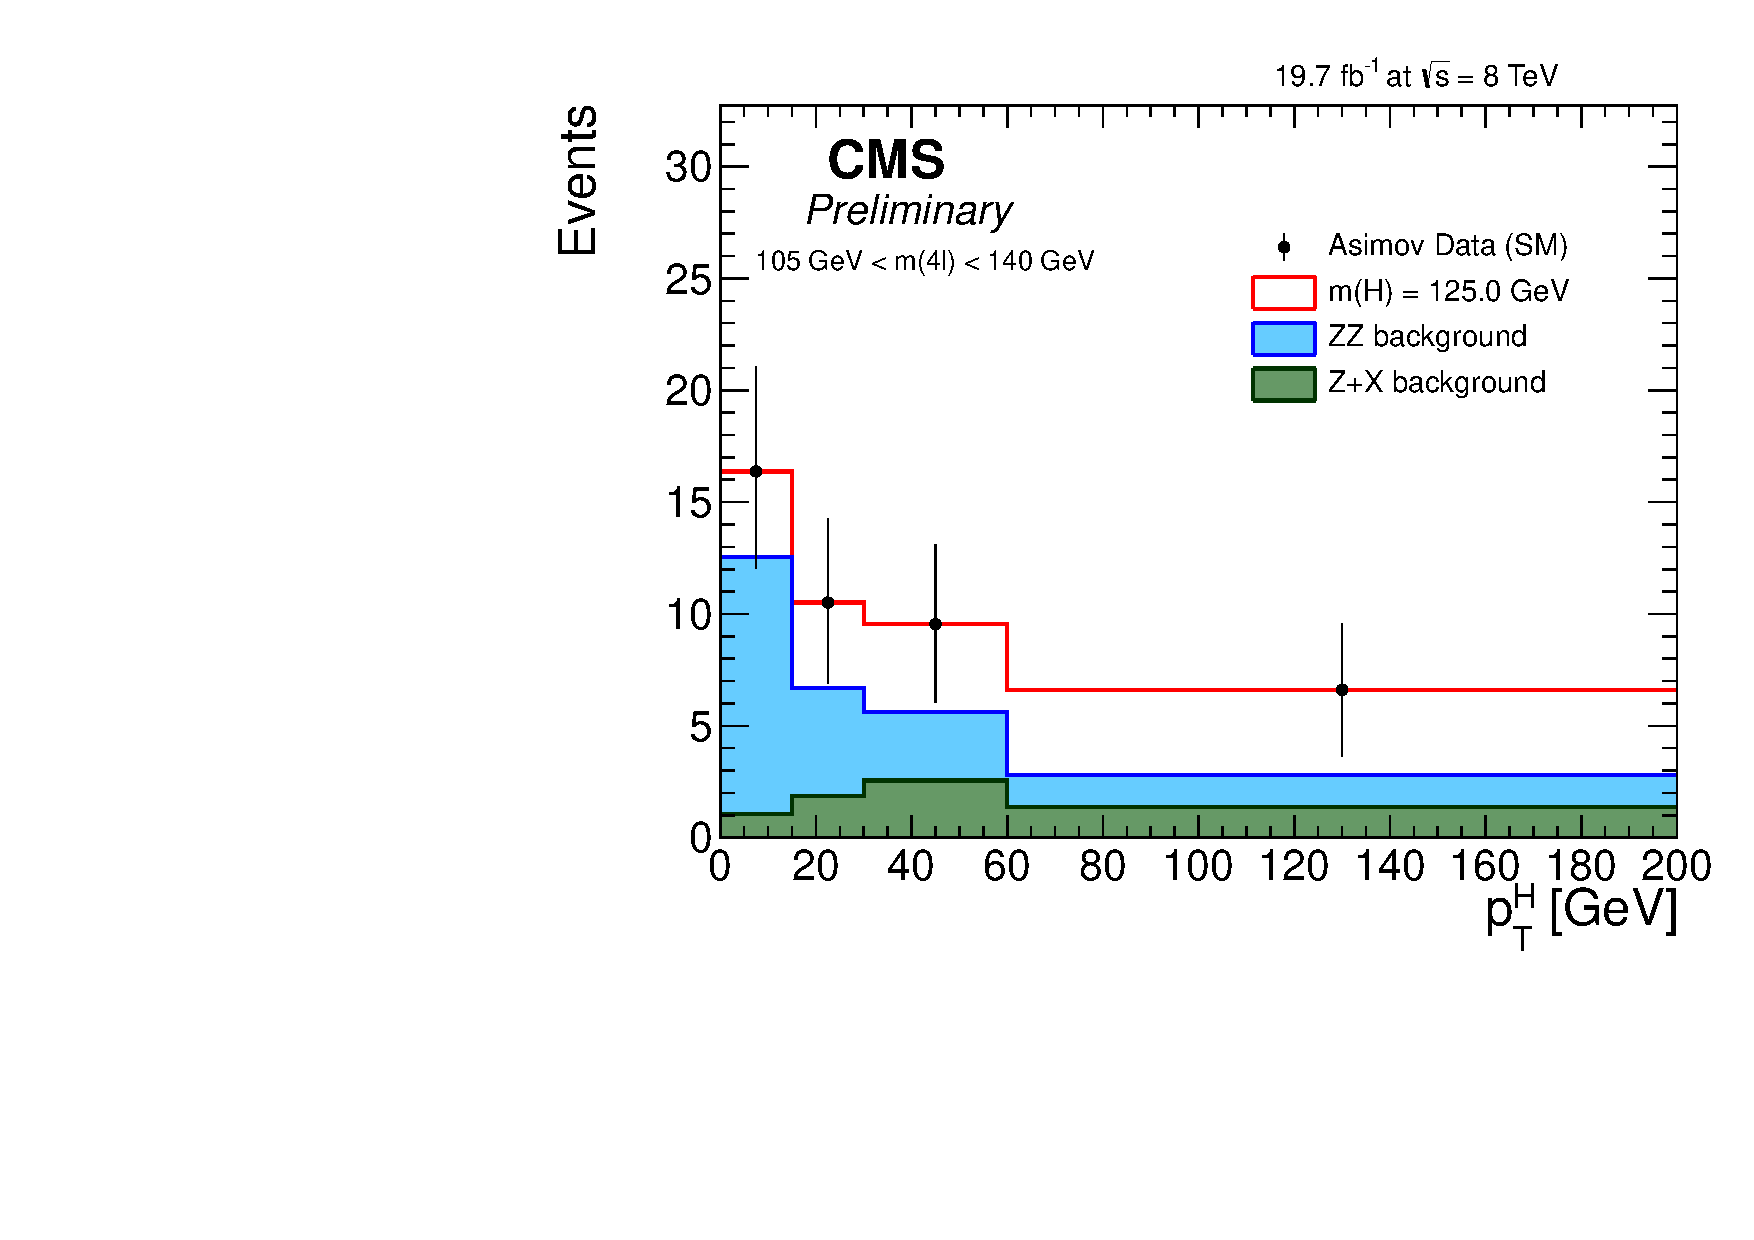
\includegraphics[width=0.42\textwidth,angle=0]{Appendix/Plots/asimovdata_SM_125_v2_pT4l_4l.pdf}
      \label{fig:differential-bins-asimov:a}
    }
    \subfigure[$|y(\mathrm{H})|$]{
      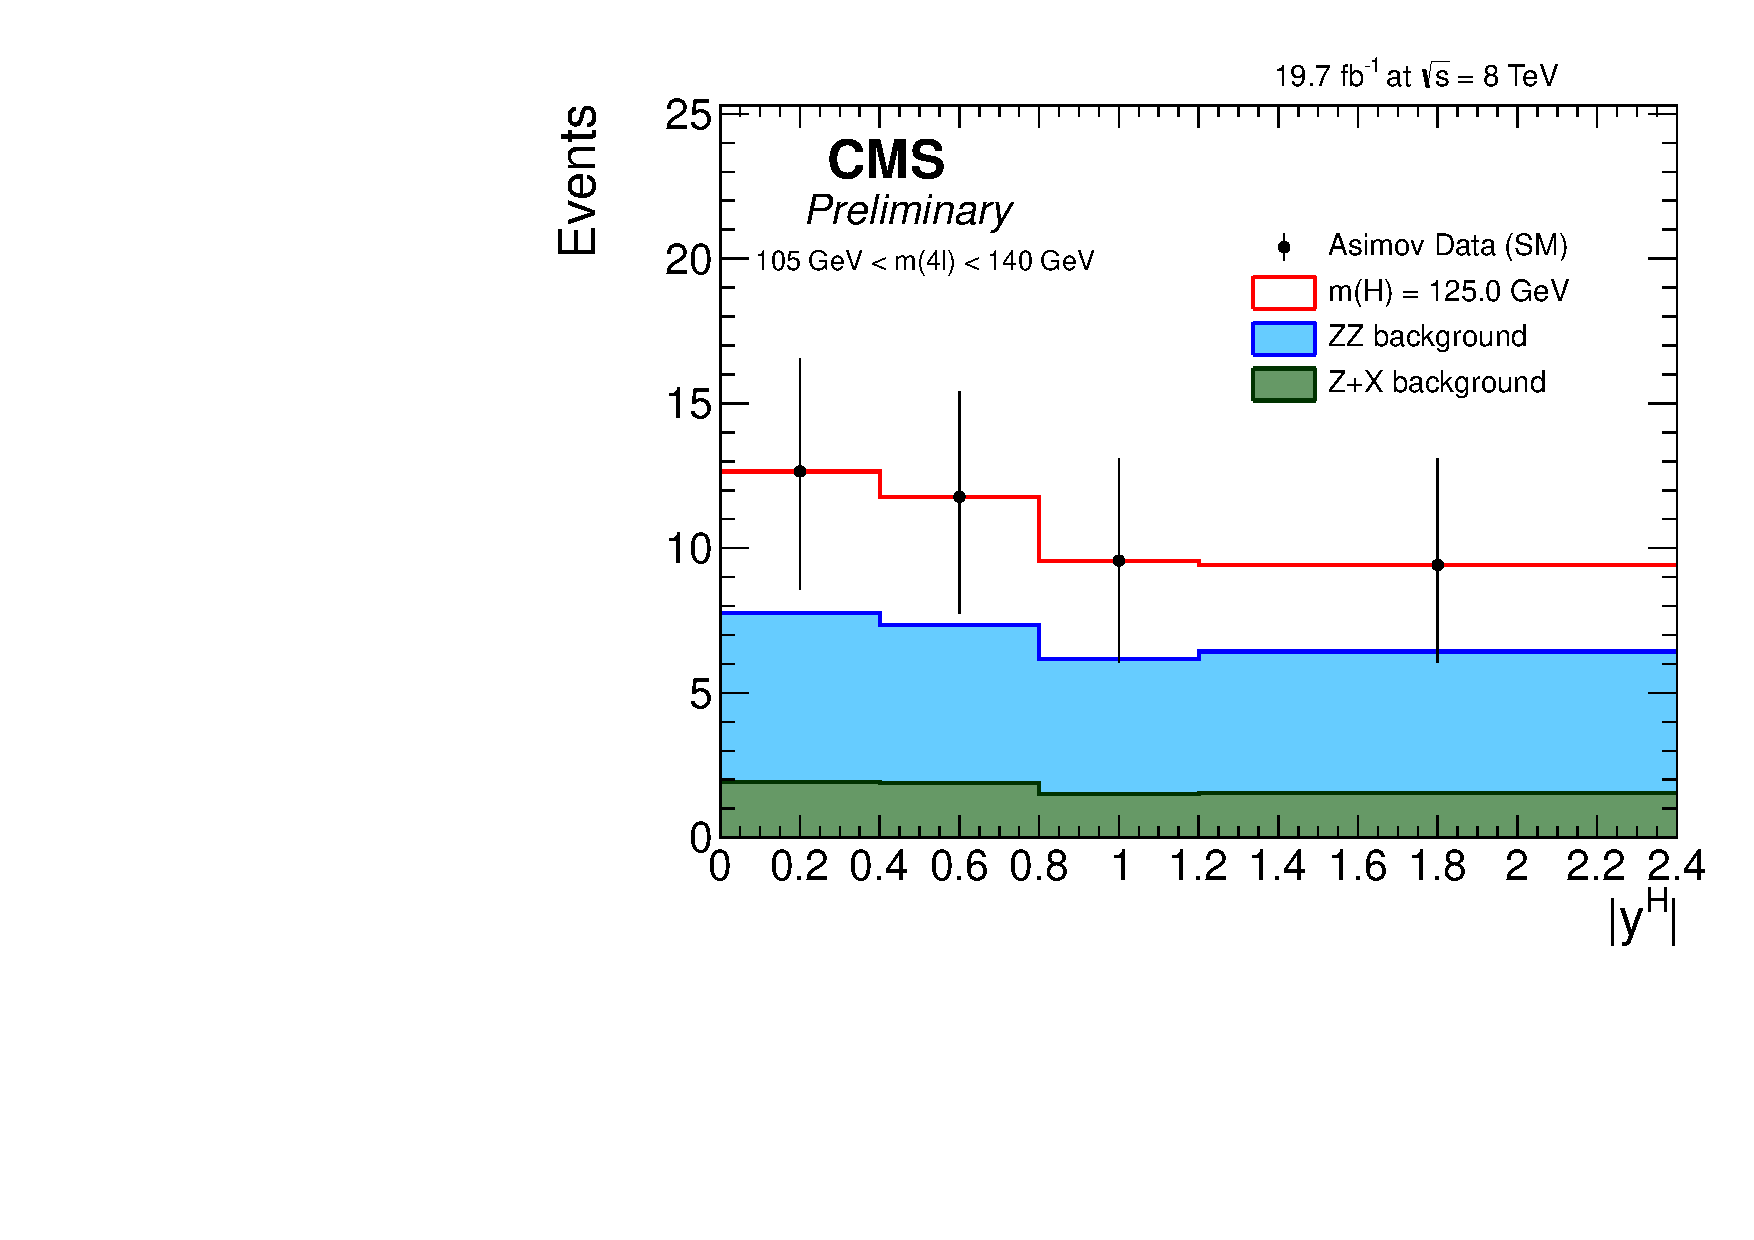
\includegraphics[width=0.42\textwidth,angle=0]{Appendix/Plots/asimovdata_SM_125_v2_rapidity4l_4l.pdf}
      \label{fig:differential-bins-asimov:b}
    } \\
    \subfigure[N(jets), $|\eta|<4.7$]{
      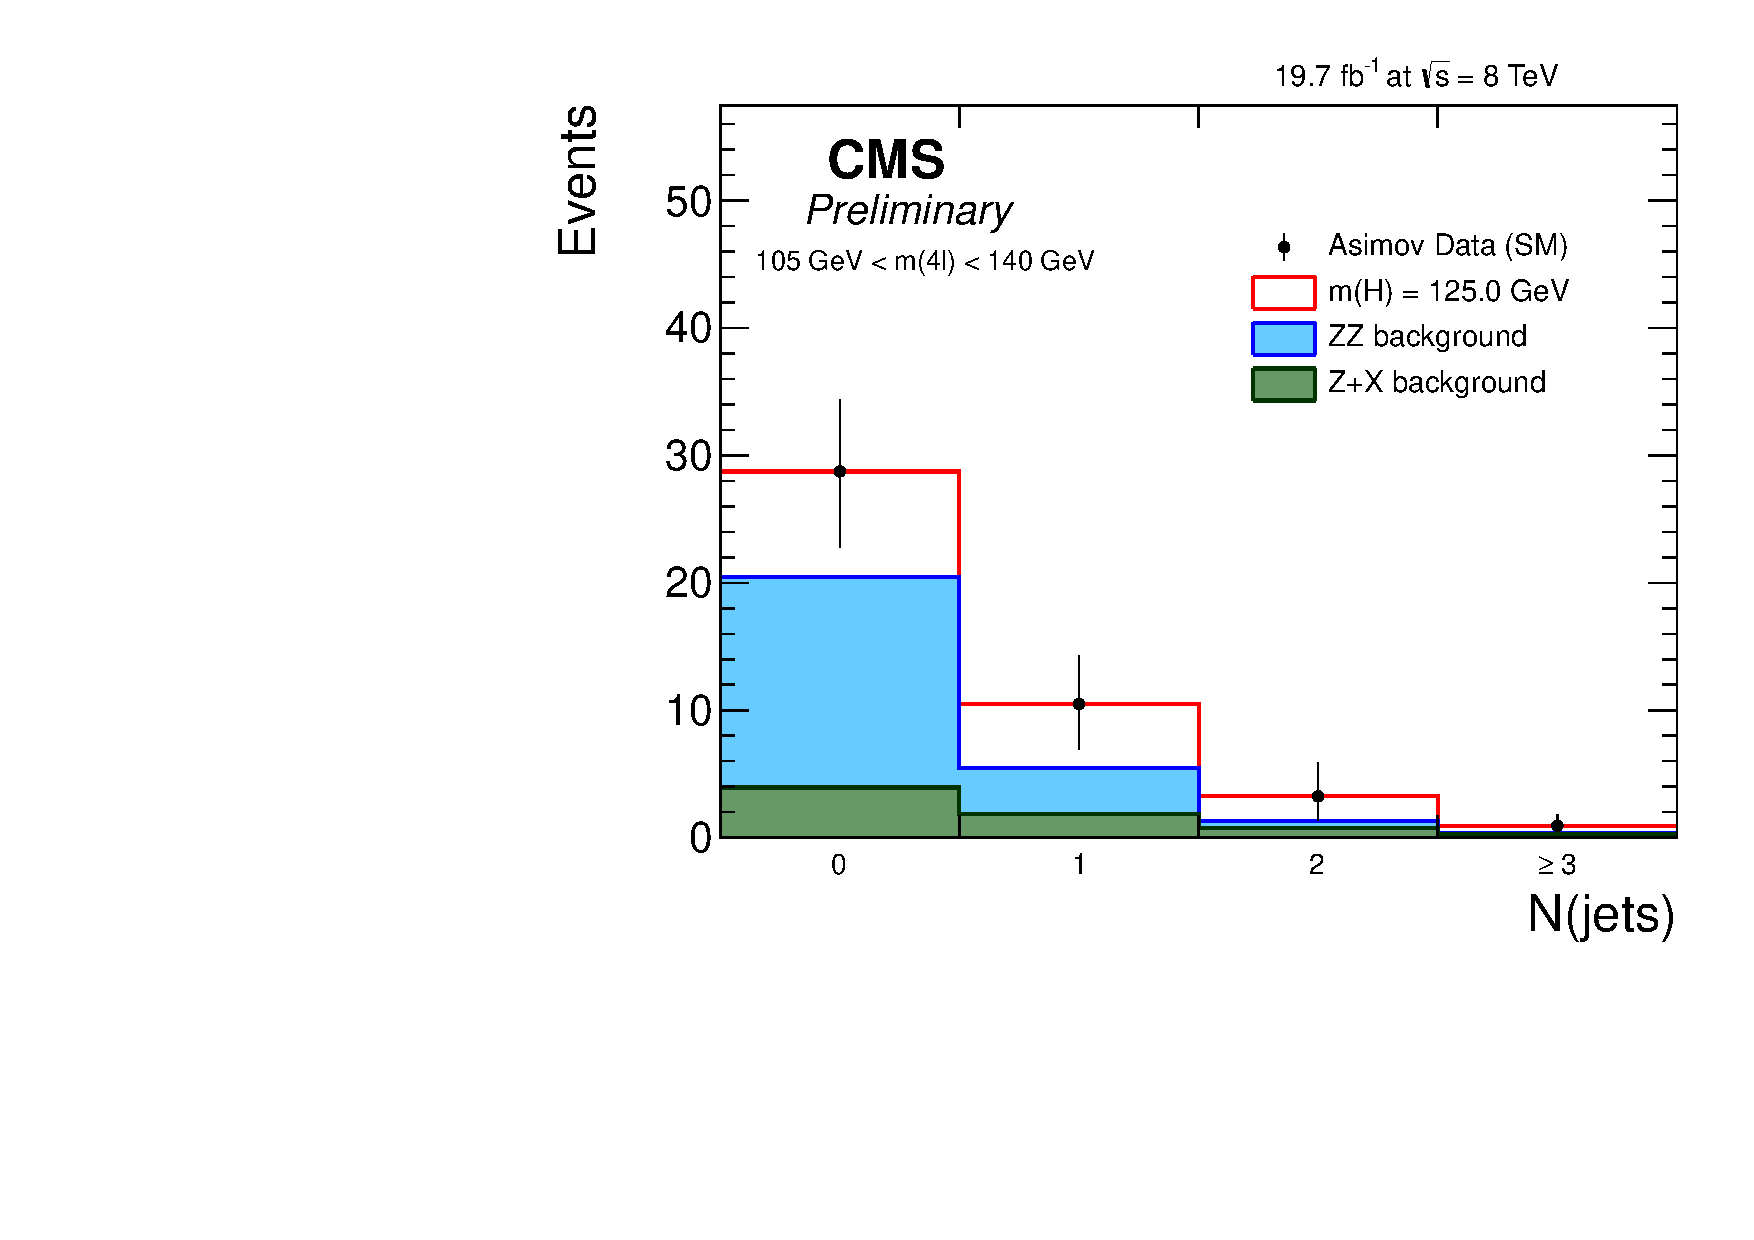
\includegraphics[width=0.42\textwidth,angle=0]{Appendix/Plots/asimovdata_SM_125_v2_njets_reco_pt30_eta4p7_4l.pdf}
      \label{fig:differential-bins-asimov:c}                                                                                                                            
    }
    \subfigure[N(jets), $|\eta|<2.5$]{
      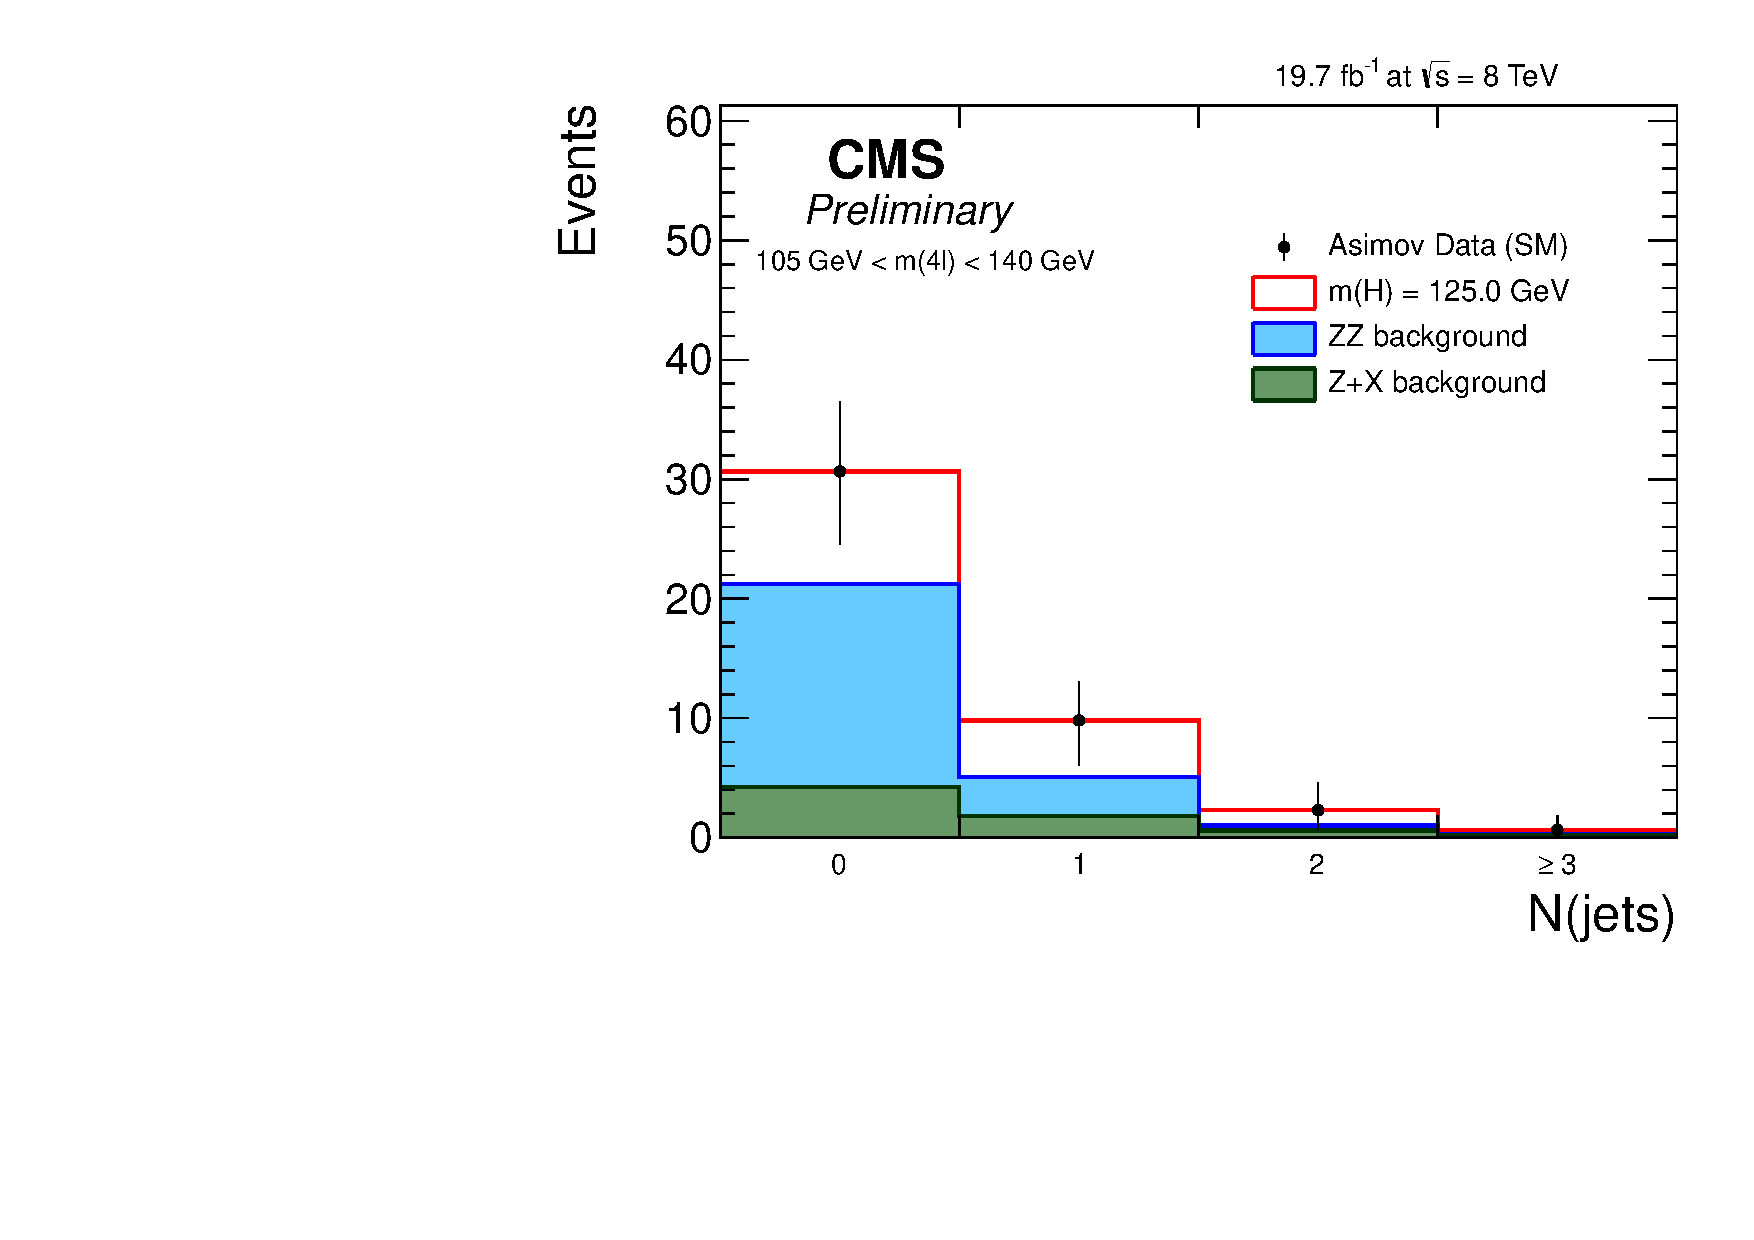
\includegraphics[width=0.42\textwidth,angle=0]{Appendix/Plots/asimovdata_SM_125_v2_njets_reco_pt30_eta2p5_4l.pdf}
      \label{fig:differential-bins-asimov:d}                                                                                                                            
    } \\
    \subfigure[$\mathrm{m}(\mathrm{Z}_{1})$]{
      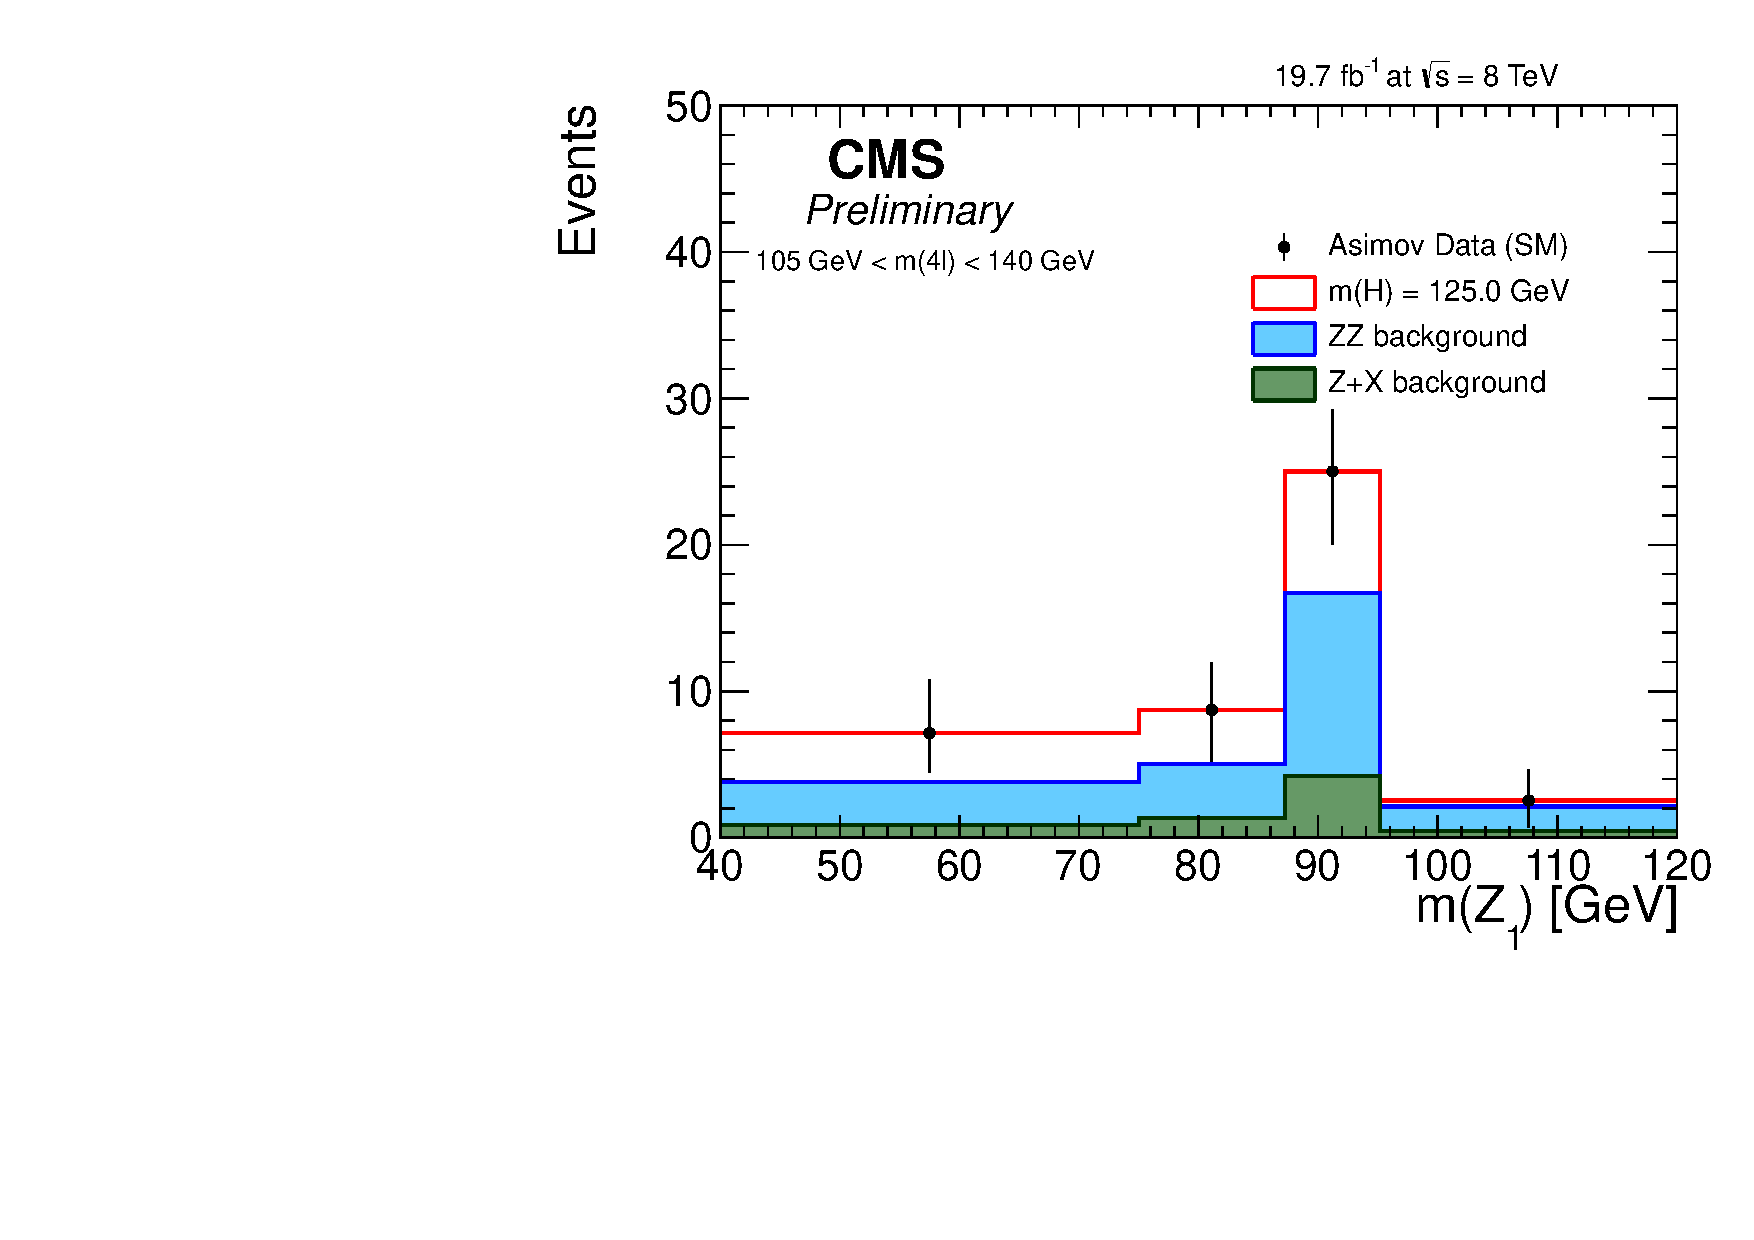
\includegraphics[width=0.42\textwidth,angle=0]{Appendix/Plots/asimovdata_SM_125_v2_massZ1_4l.pdf}
      \label{fig:differential-bins-asimov:e}
    }
    \subfigure[$\mathrm{m}(\mathrm{Z}_{2})$]{
      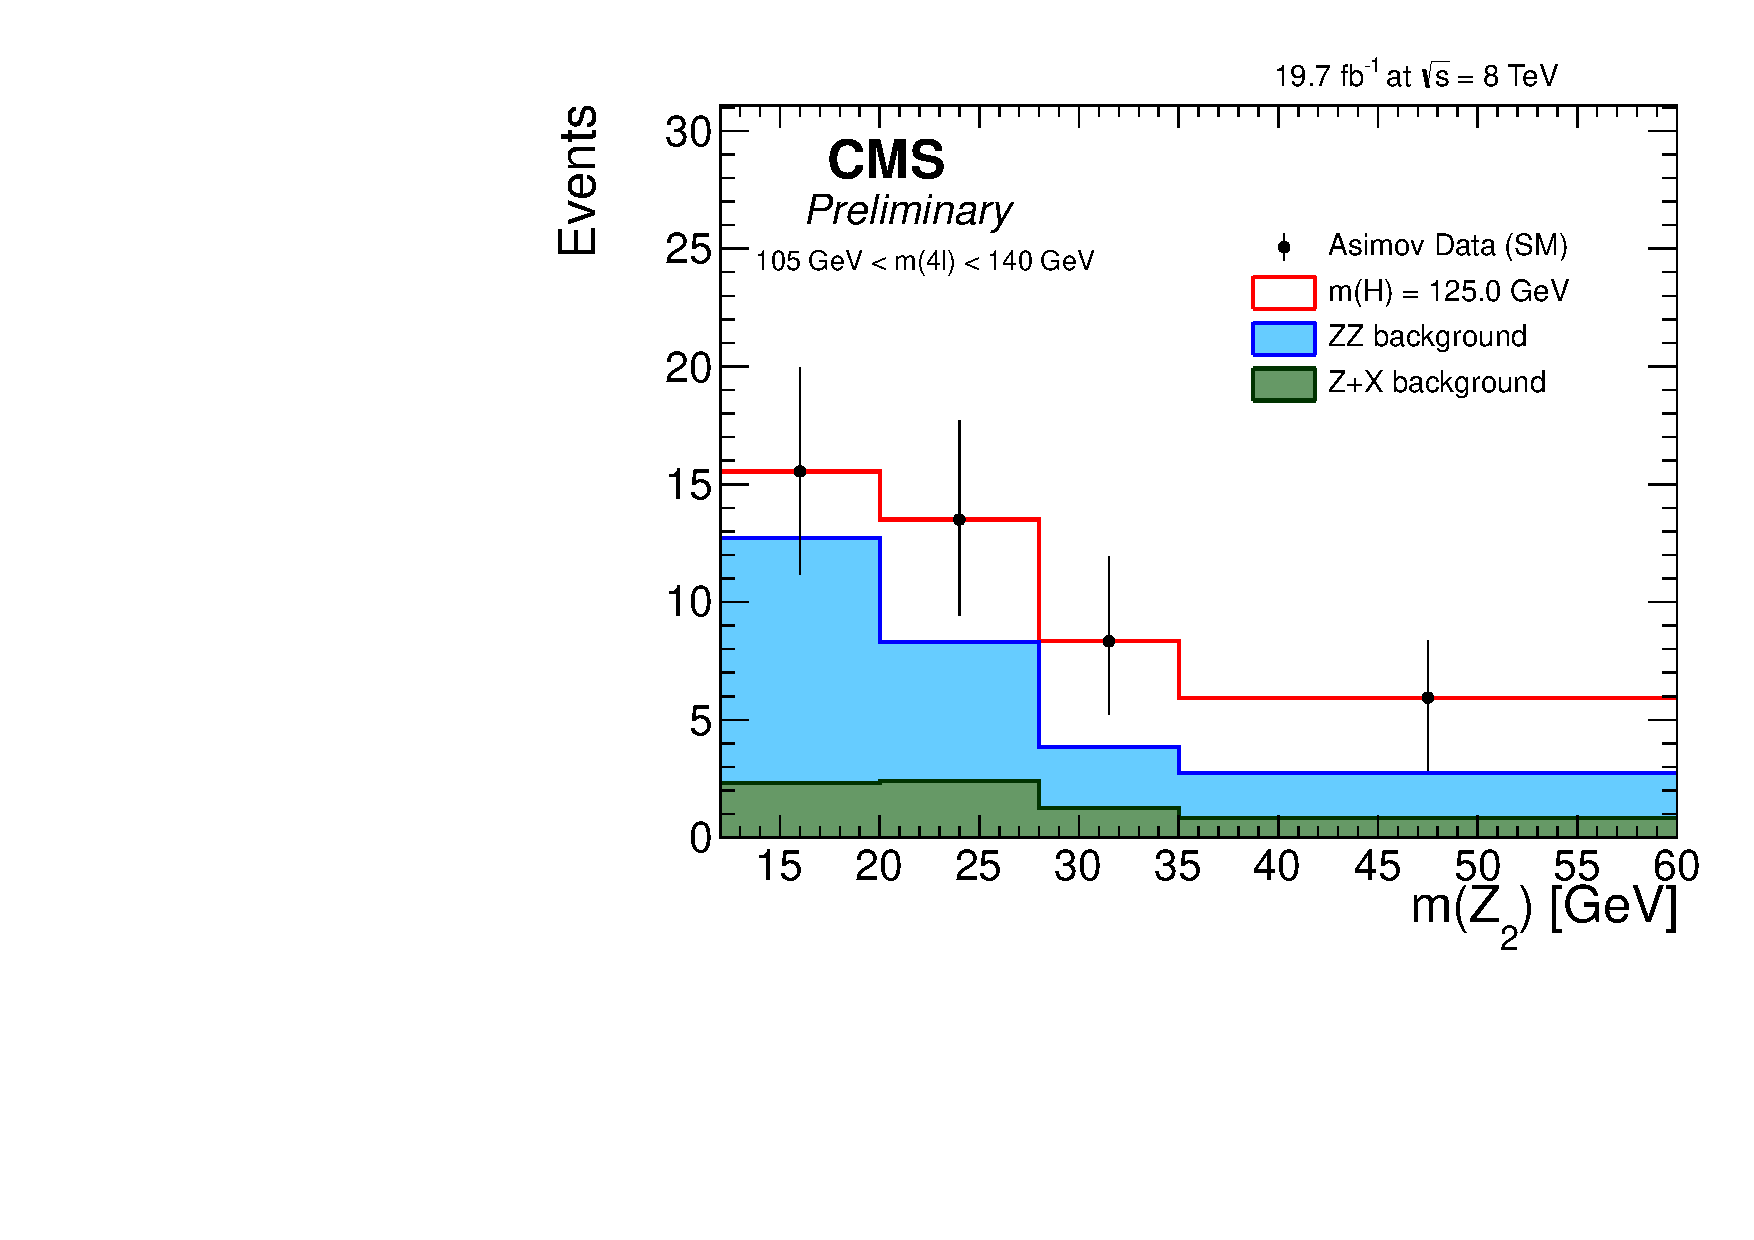
\includegraphics[width=0.42\textwidth,angle=0]{Appendix/Plots/asimovdata_SM_125_v2_massZ2_4l.pdf}
      \label{fig:differential-bins-asimov:f}
    }
    \caption{Observed data along with the SM signal (m(H)=$125.0 \GeV$) and background expectations for different observables and for all final states combined, in range $105 < m_{4\ell} < 140 \GeV$ used for the $\Hllll$ measurements. The extraction of the signal is performed by exploiting the differences in the expected $m_{4\ell}$ spectra of the signal and background contributions in each bin of an observable.
    COMMENT: Results shown with Asimov dataset.
    }
  \label{fig:differential-bins-asimov}
 \end{center}
\end{figure}


\begin{figure}[!h!t]
  \begin{center}
    \subfigure[$|\cos \theta_{1}|$]{
      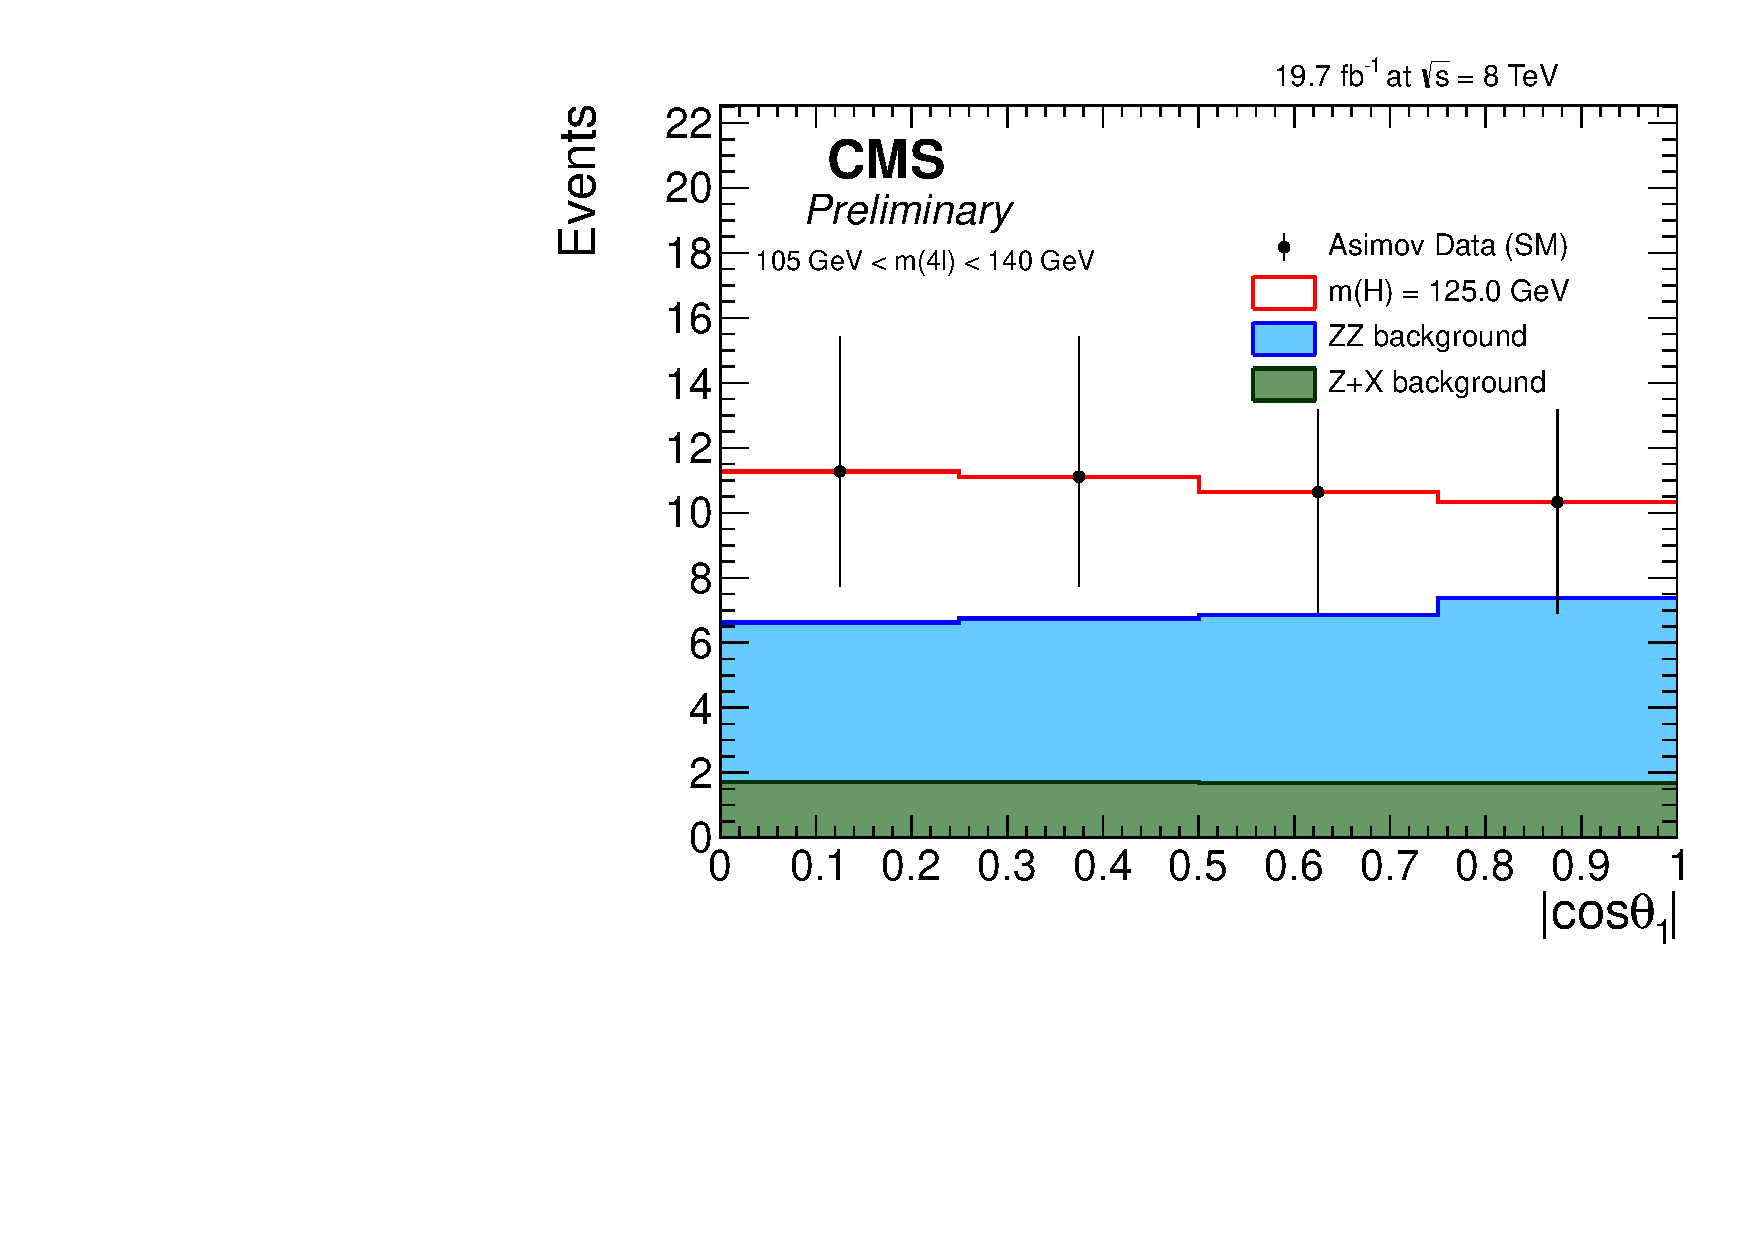
\includegraphics[width=0.42\textwidth,angle=0]{Appendix/Plots/asimovdata_SM_125_v2_cosTheta1_4l.pdf}
      \label{fig:differential-bins-asimov-2:a}
    }
    \subfigure[$|\cos \theta_{2}|$]{
      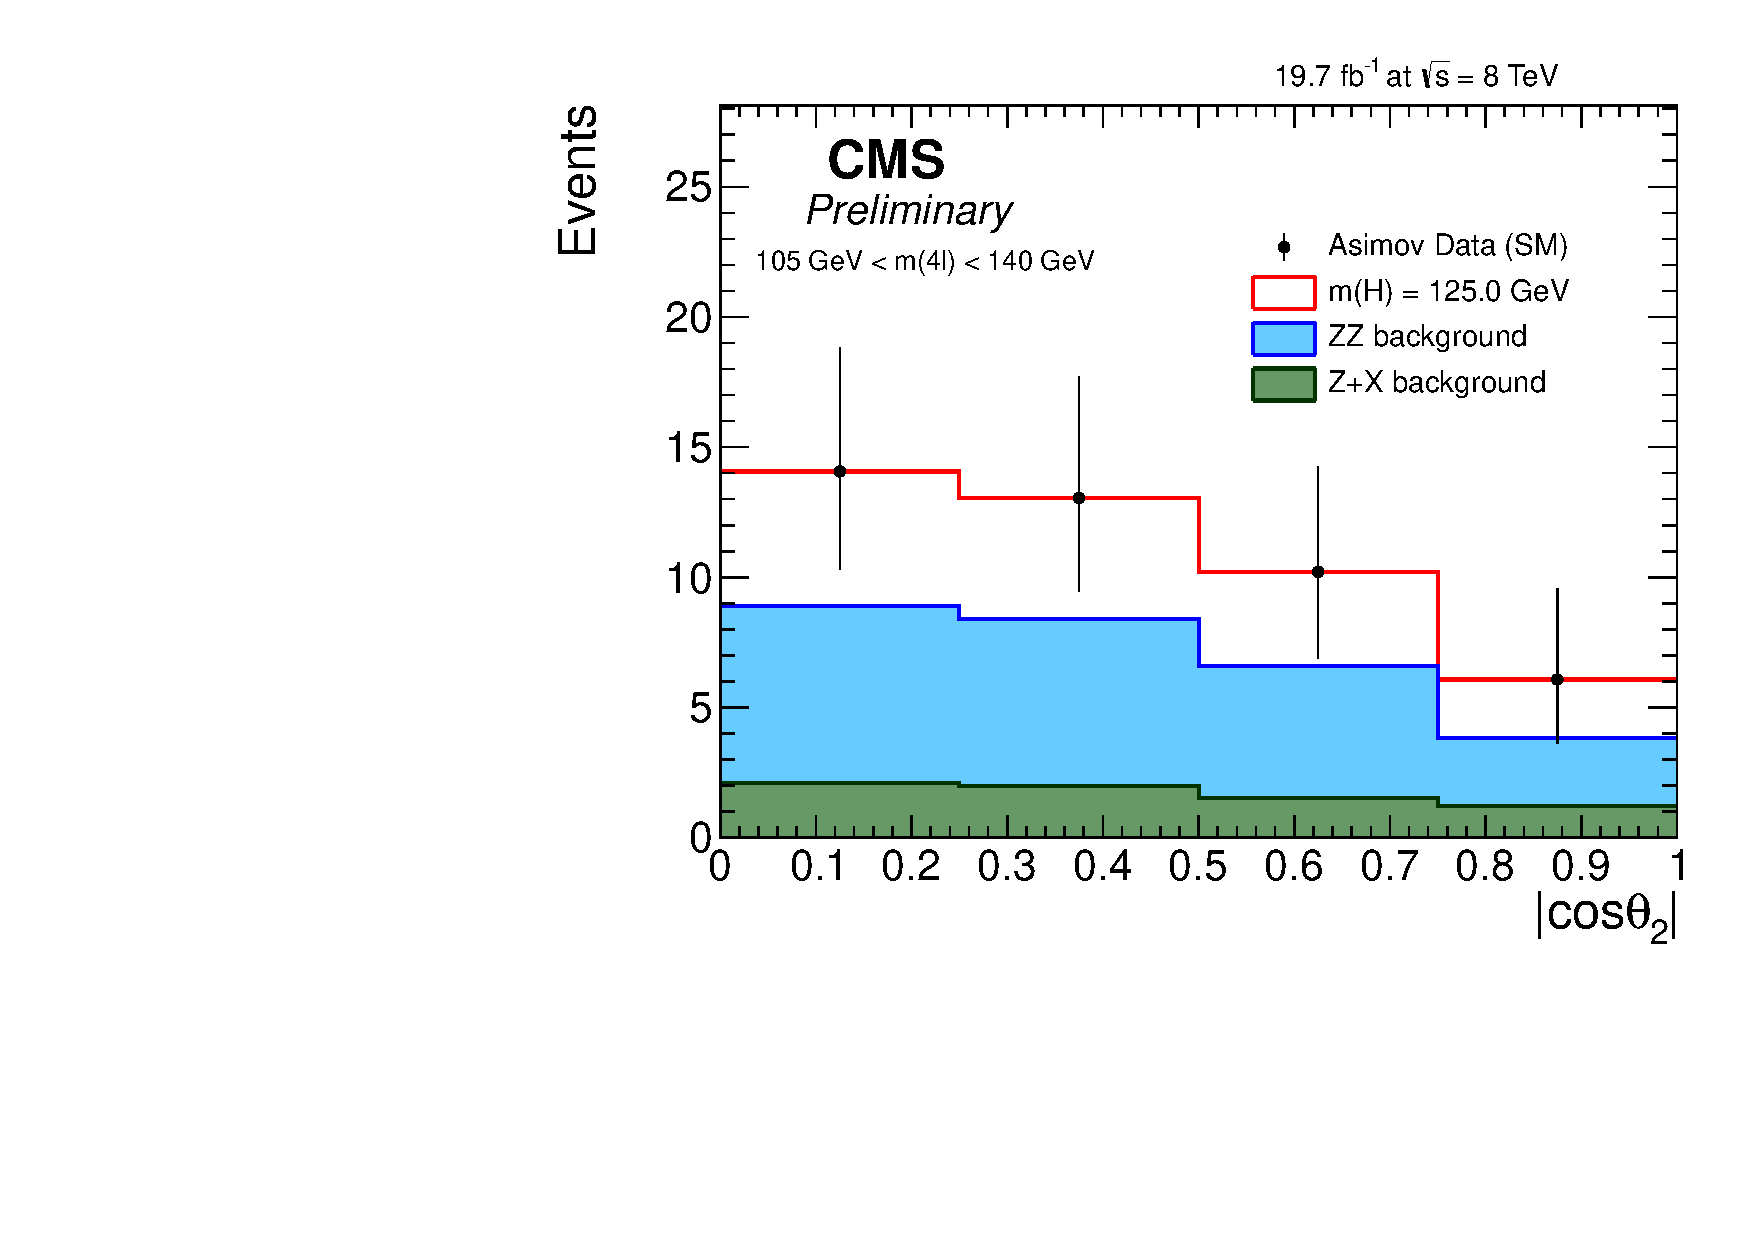
\includegraphics[width=0.42\textwidth,angle=0]{Appendix/Plots/asimovdata_SM_125_v2_cosTheta2_4l.pdf}
      \label{fig:differential-bins-asimov-2:b}
    } \\
    \subfigure[$|\Phi|$]{
      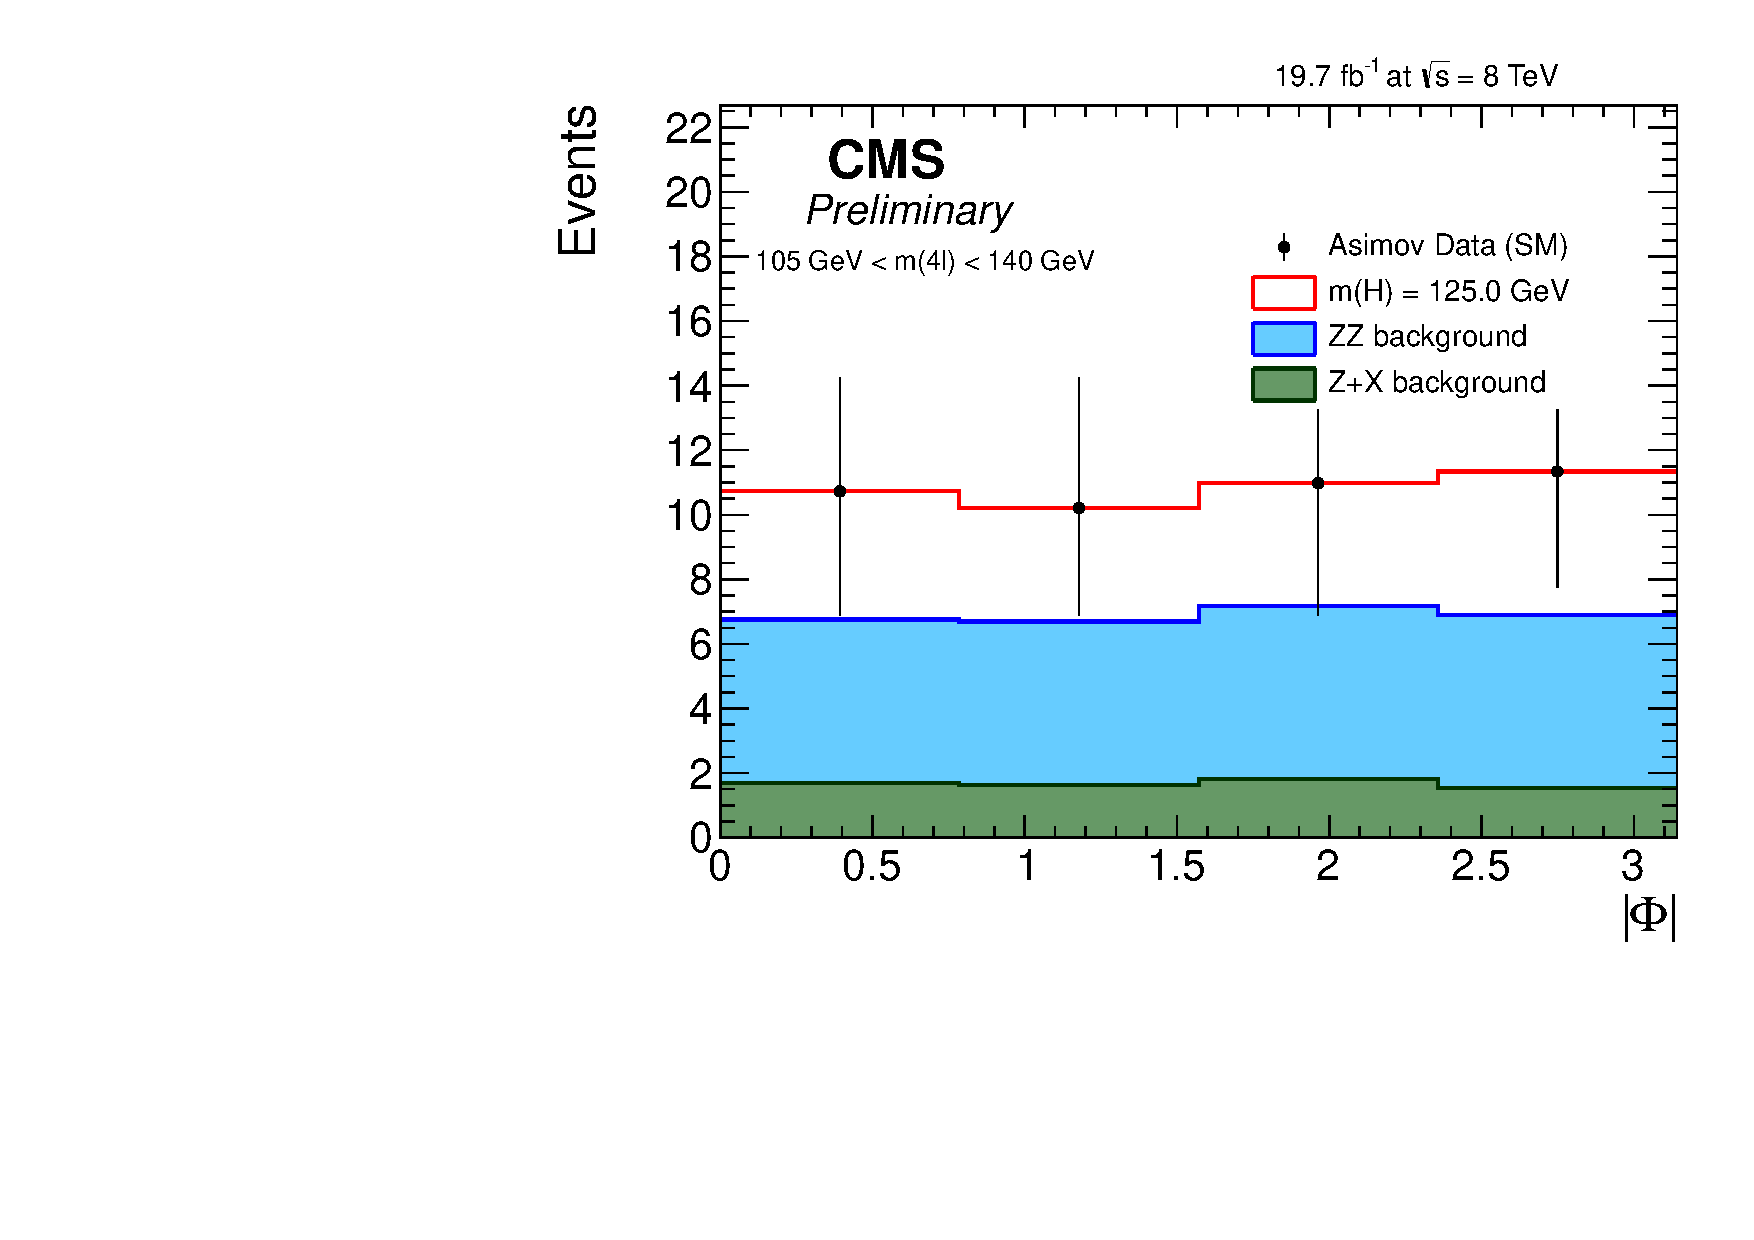
\includegraphics[width=0.42\textwidth,angle=0]{Appendix/Plots/asimovdata_SM_125_v2_Phi_4l.pdf}
      \label{fig:differential-bins-asimov-2:c}
    }
    \subfigure[$|\Phi_{1}|$]{
      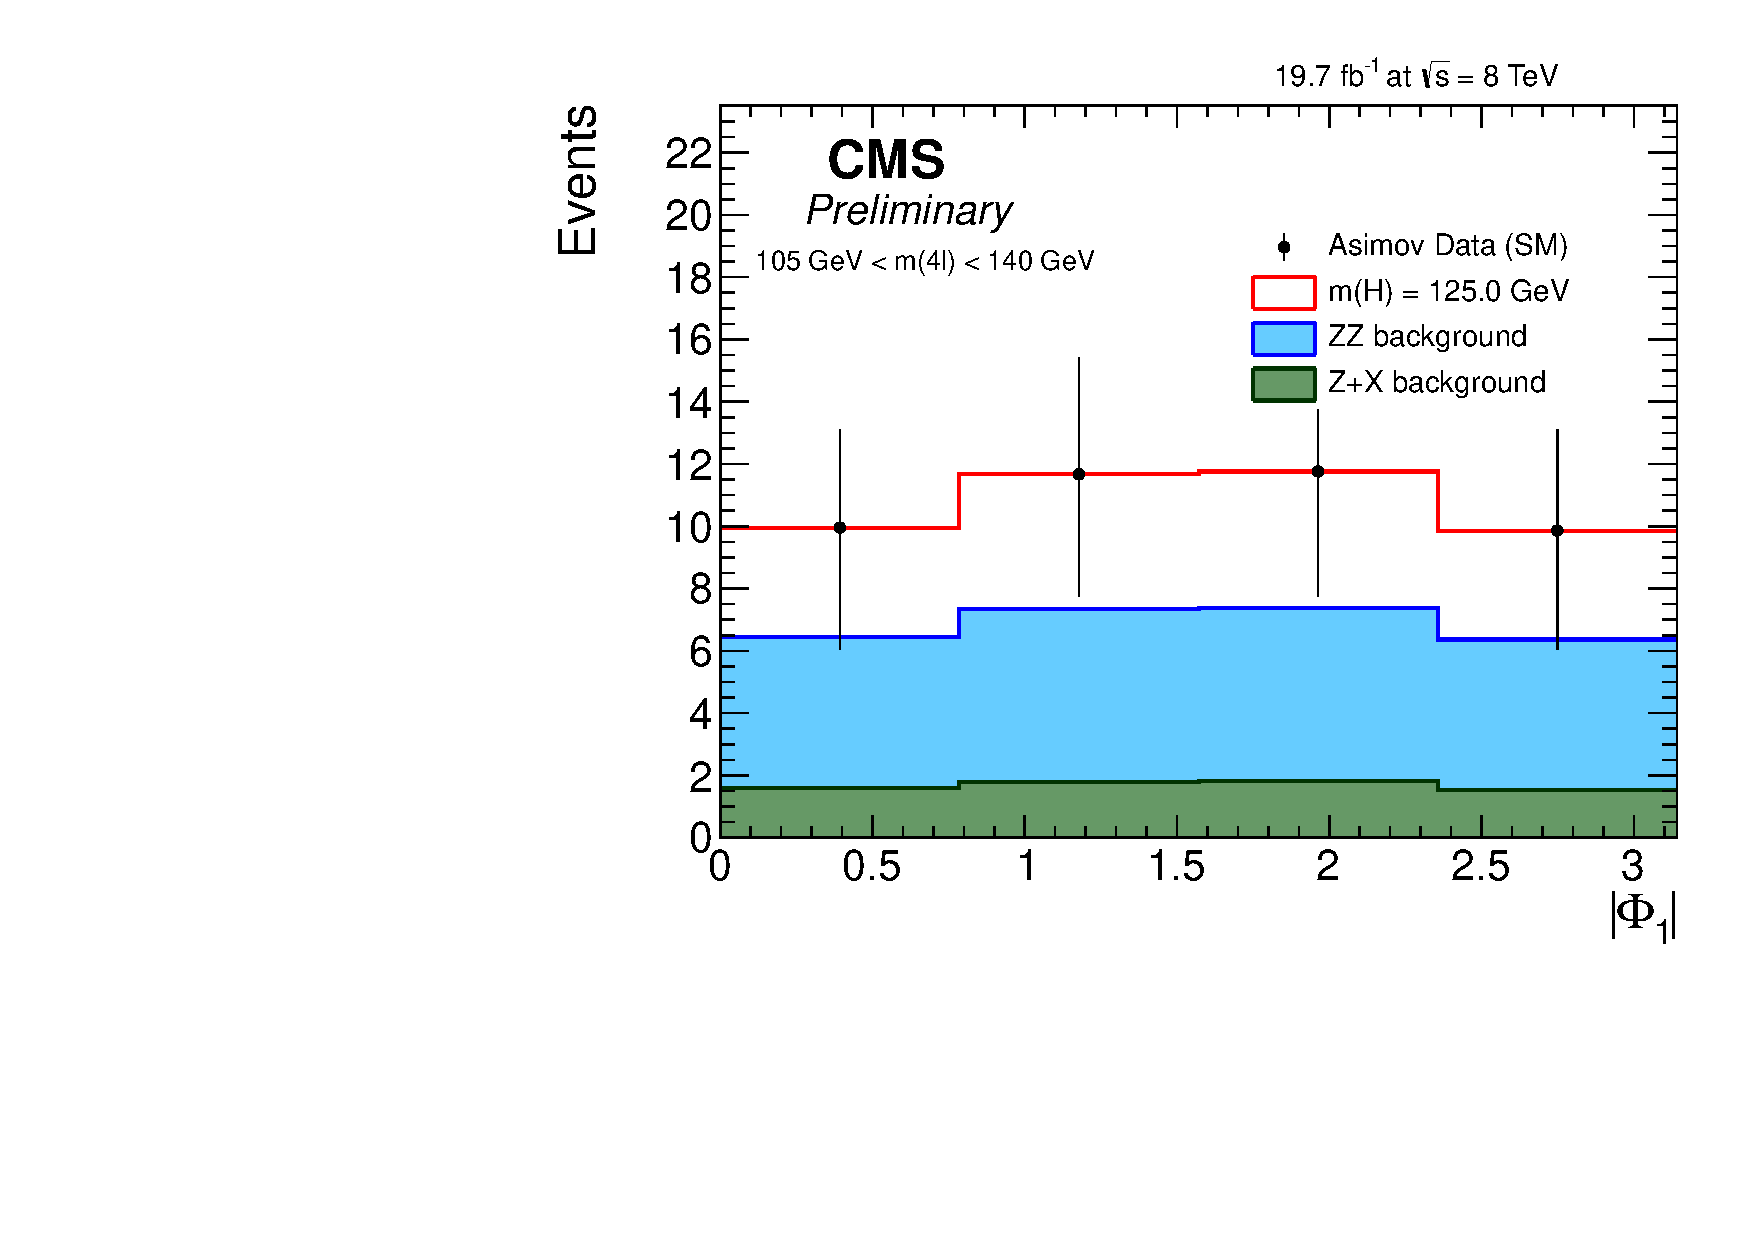
\includegraphics[width=0.42\textwidth,angle=0]{Appendix/Plots/asimovdata_SM_125_v2_Phi1_4l.pdf}
      \label{fig:differential-bins-asimov-2:d}
    } \\
    \subfigure[$|\cos \theta^{*}|$]{
      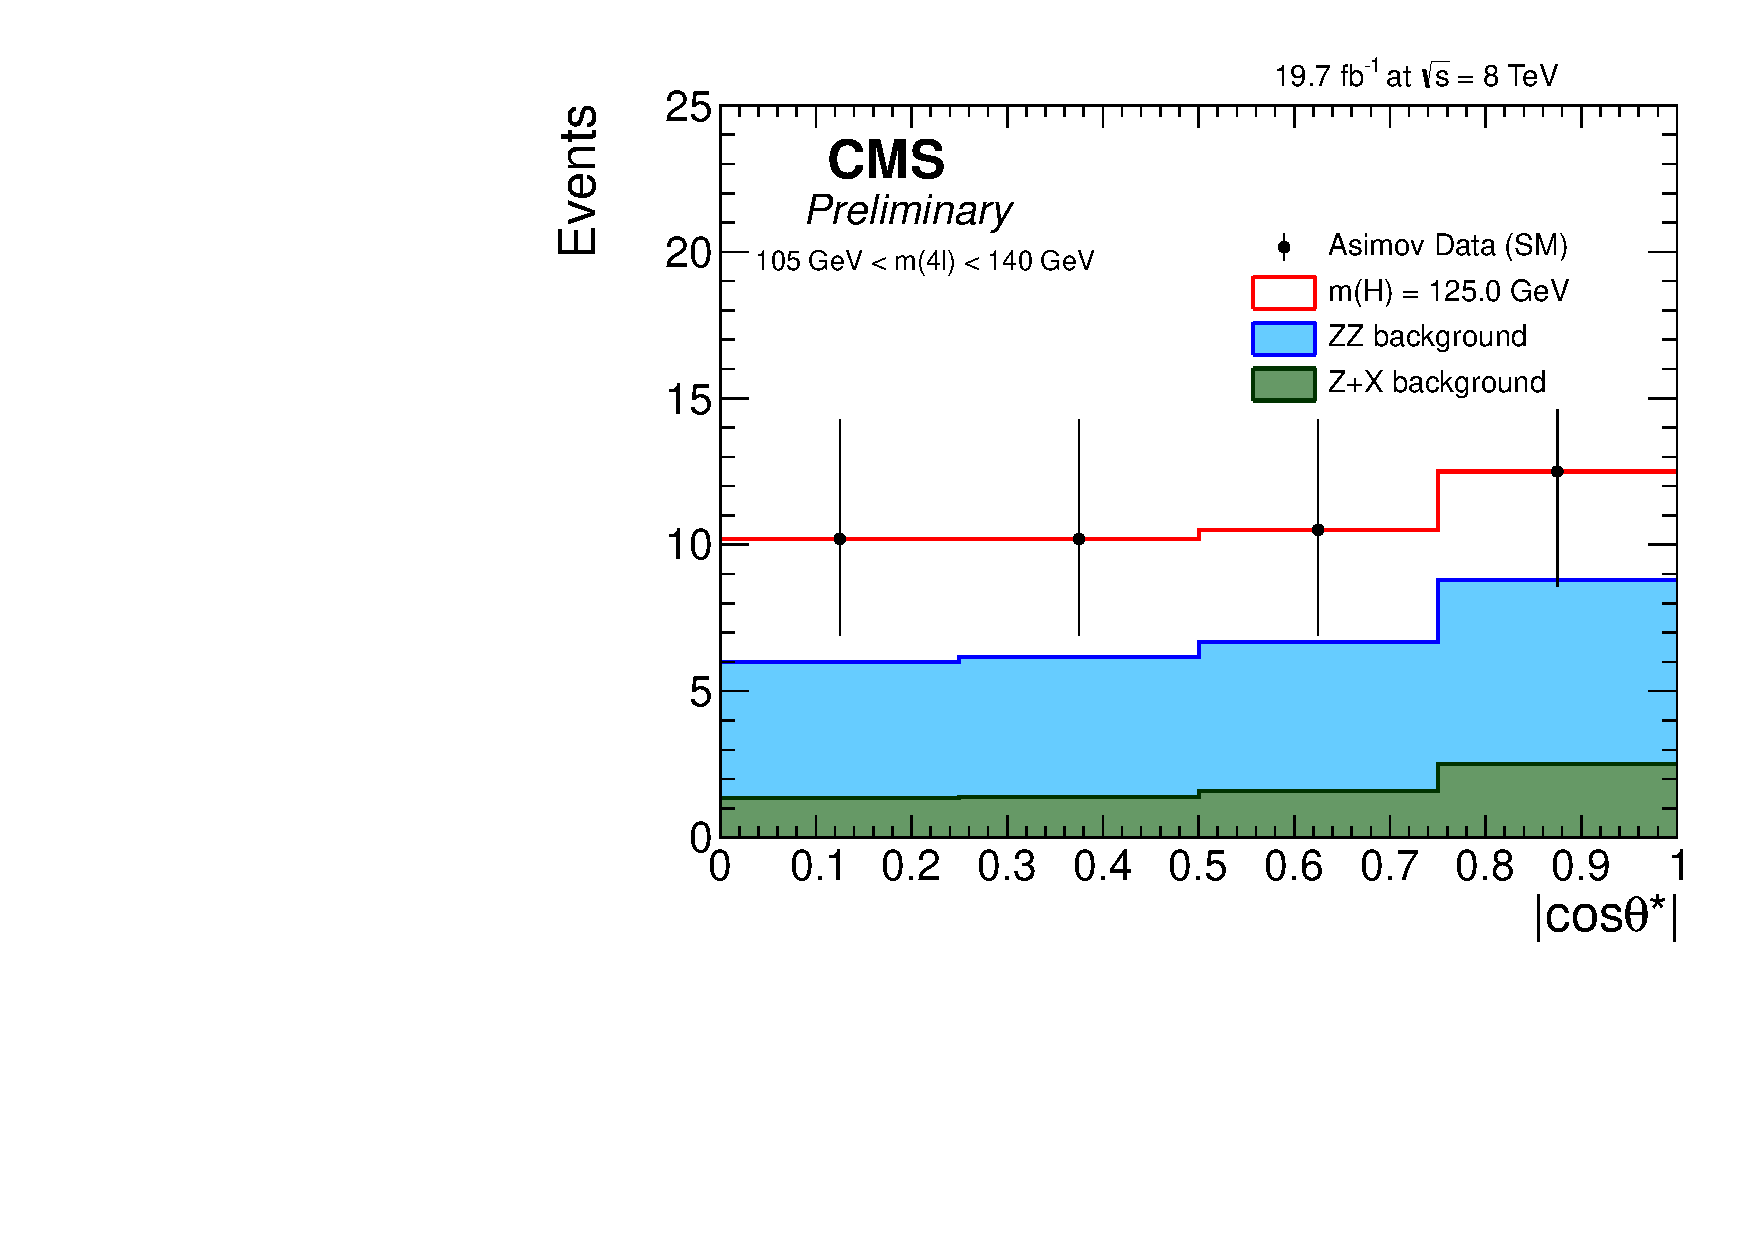
\includegraphics[width=0.42\textwidth,angle=0]{Appendix/Plots/asimovdata_SM_125_v2_cosThetaStar_4l.pdf}
      \label{fig:differential-bins-asimov-2:e}
    }
    \caption{Observed data along with the SM signal (m(H)=$125.0 \GeV$) and background expectations for different observables and for all final states combined, in range $105 < m_{4\ell} < 140 \GeV$ used for the $\Hllll$ measurements. The extraction of the signal is performed by exploiting the differences in the expected $m_{4\ell}$ spectra of the signal and background contributions in each bin of an observable. 
    COMMENT: Results shown with Asimov dataset.
    }
  \label{fig:differential-bins-asimov-2}
 \end{center}
\end{figure}

\begin{figure}[!h!t]
  \begin{center}

    \subfigure[$\pt(\mathrm{H})$]{
      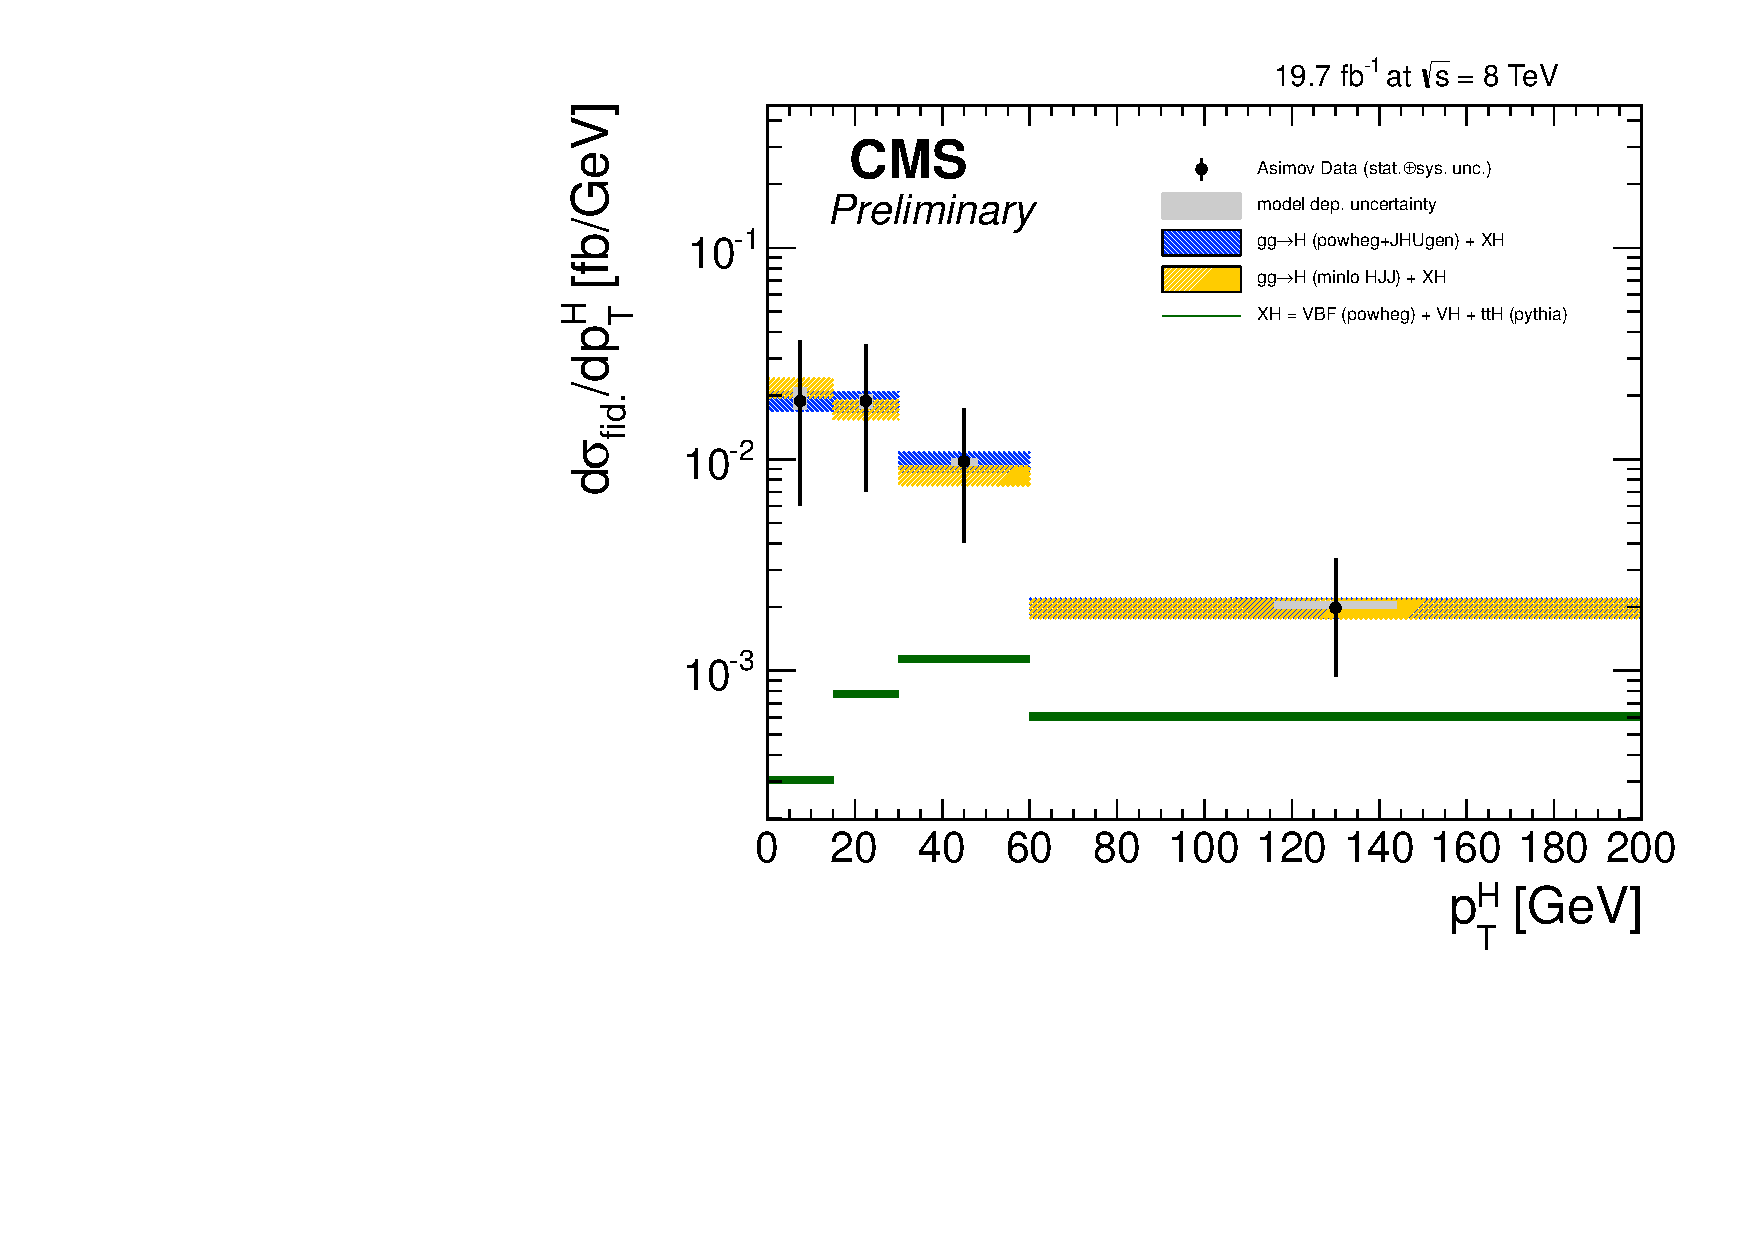
\includegraphics[width=0.42\textwidth,angle=0]{Appendix/Plots/pT4l_unfoldwith_SM_125_logscale.pdf}
      \label{fig:differential-results-asimov:a}
    }
    \subfigure[$|y(\mathrm{H})|$]{
      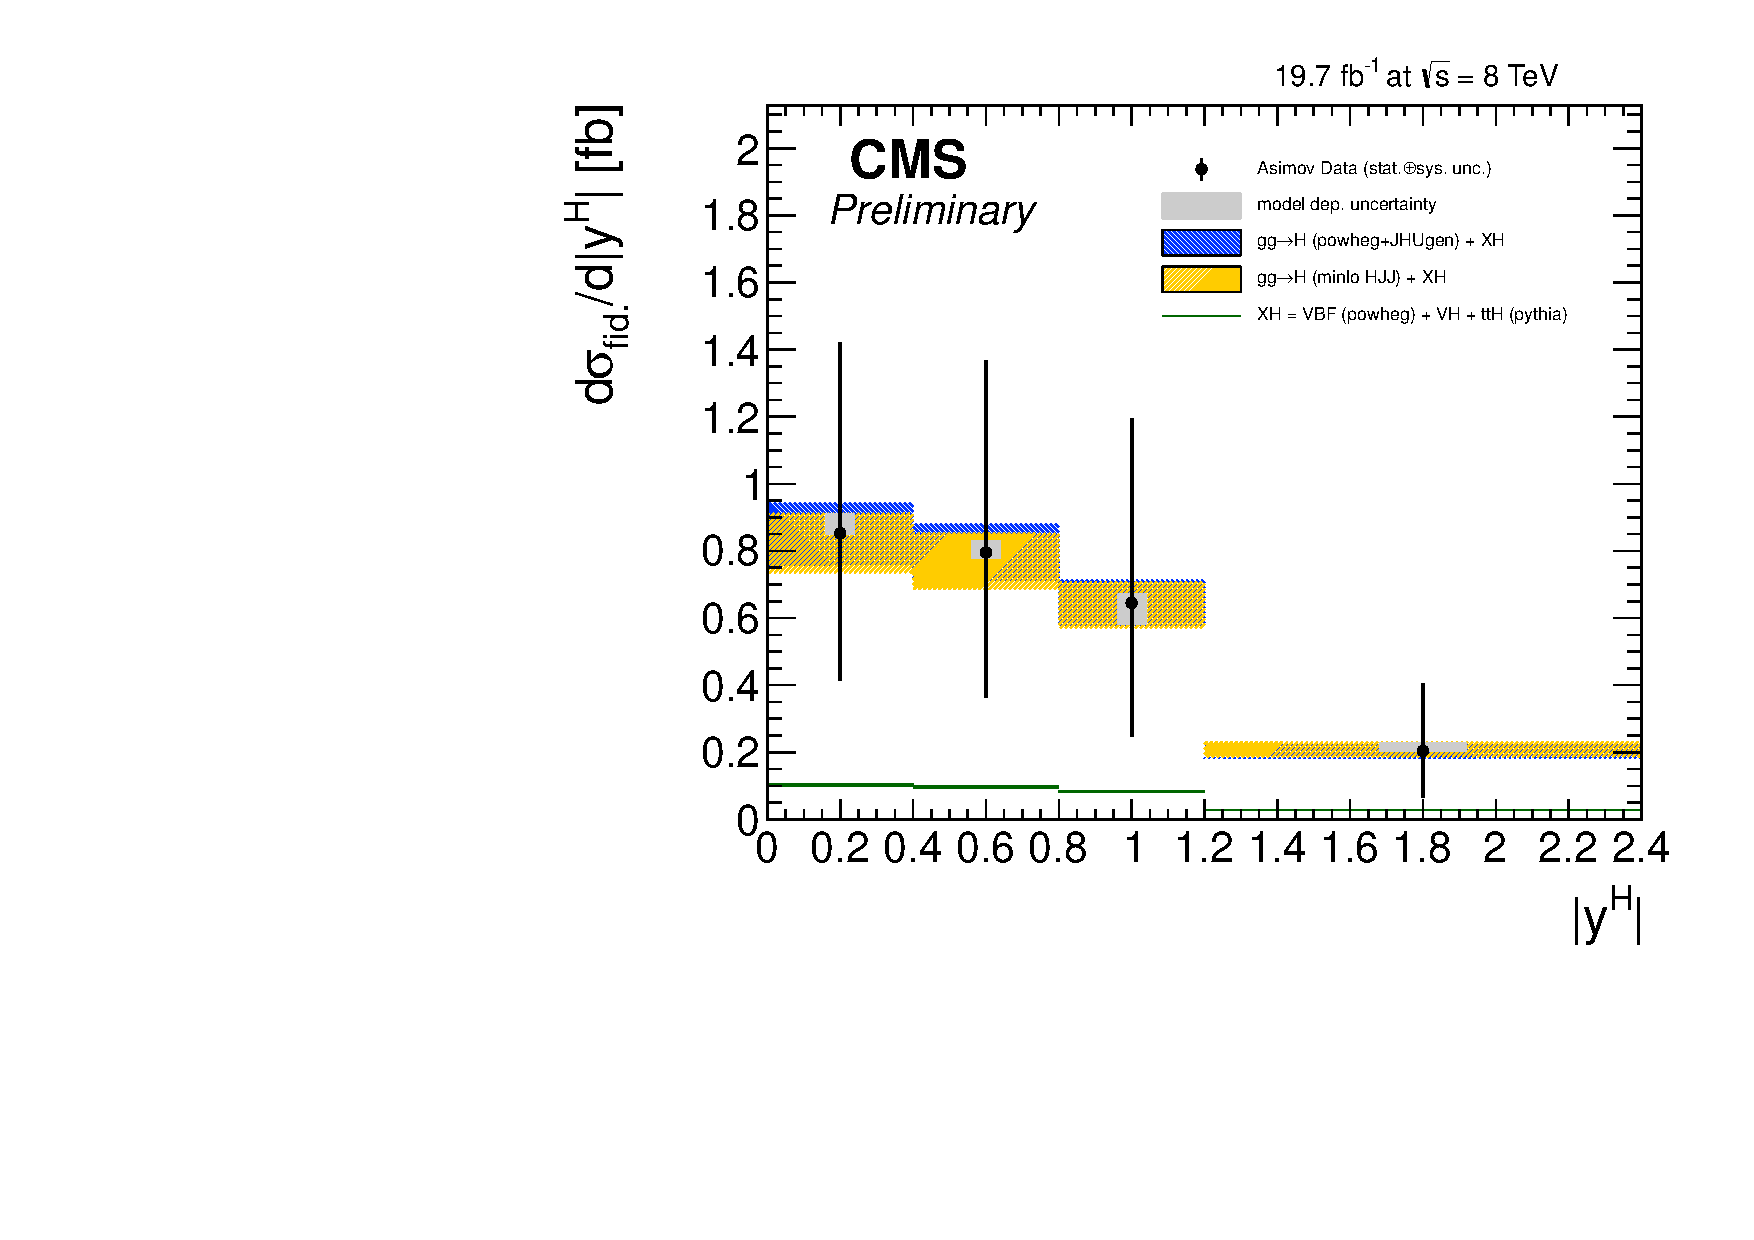
\includegraphics[width=0.42\textwidth,angle=0]{Appendix/Plots/rapidity4l_unfoldwith_SM_125.pdf}
      \label{fig:differential-results-asimov:b}
    } \\
    \subfigure[$\mathrm{m}(\mathrm{Z}_{1})$]{
      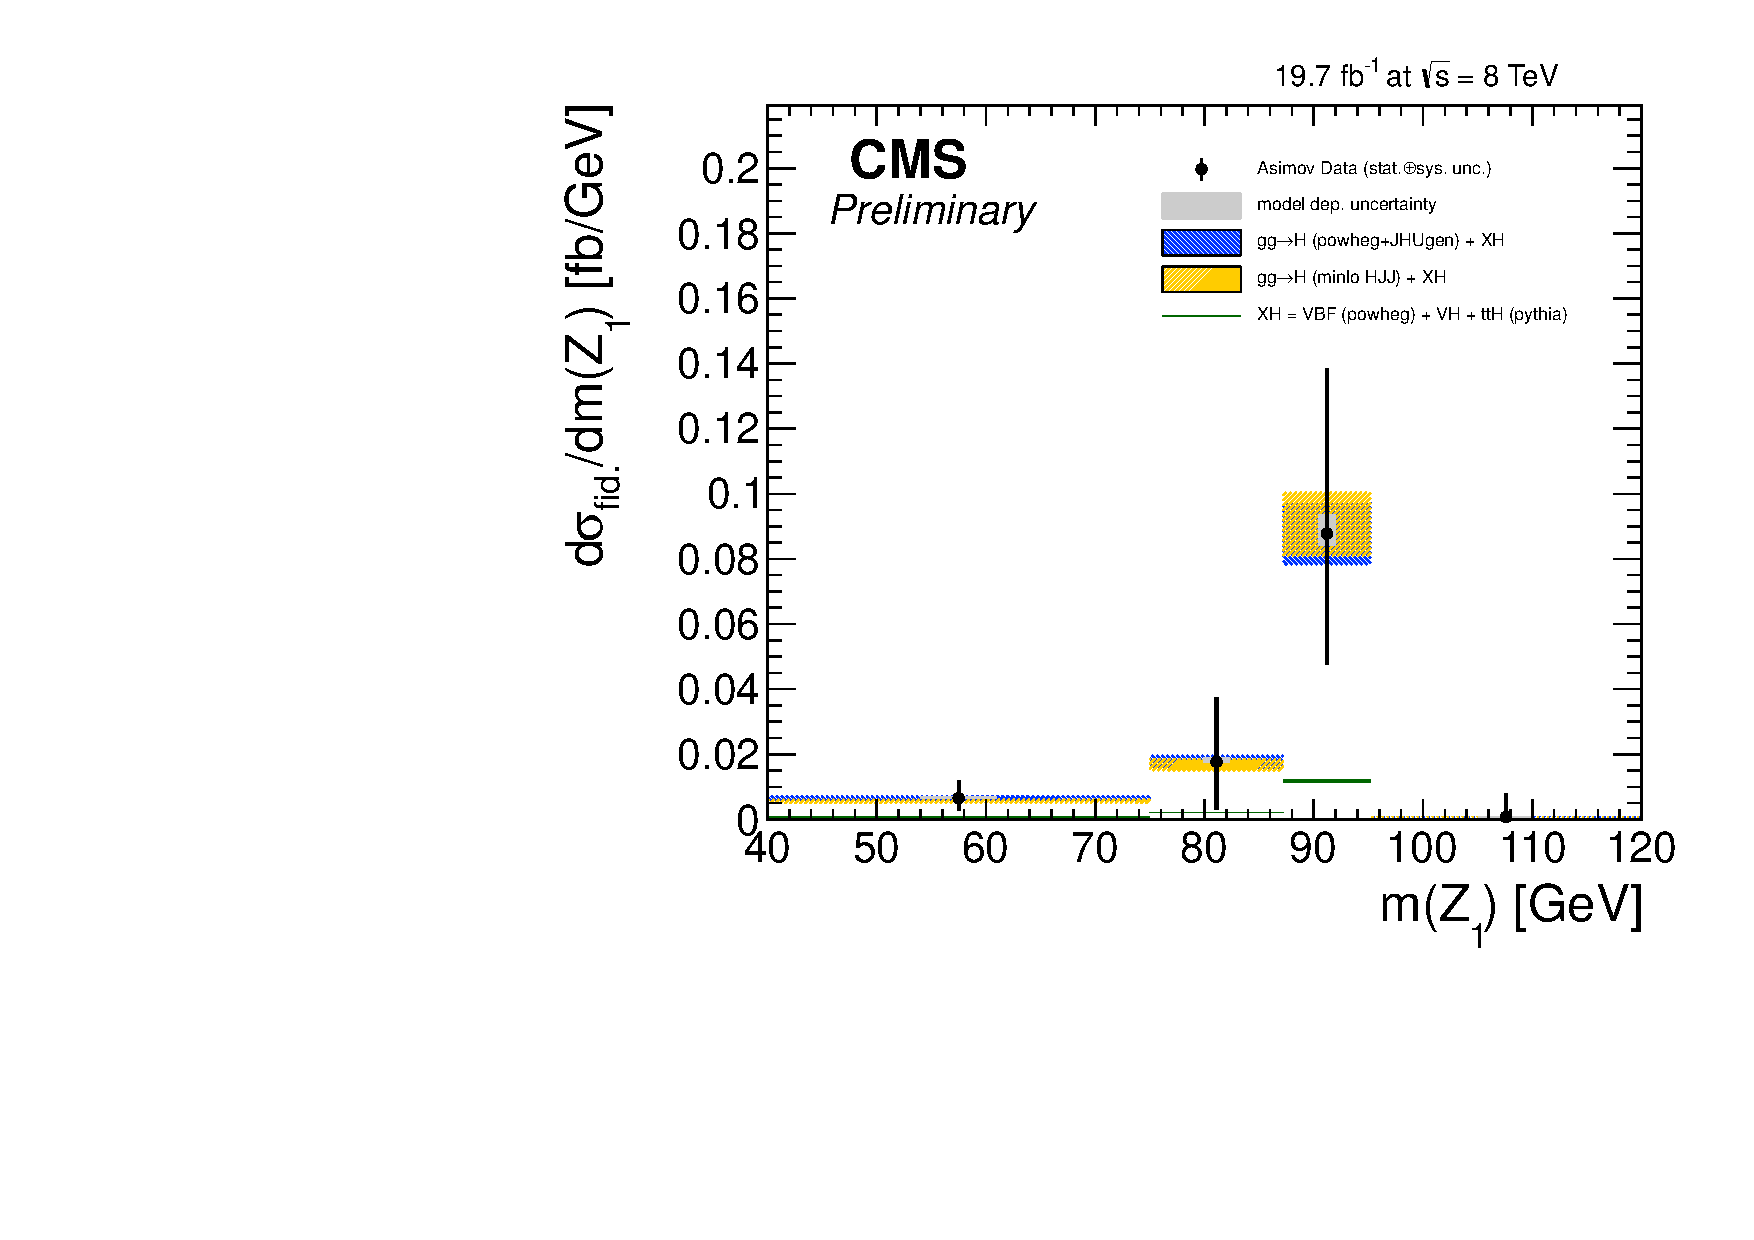
\includegraphics[width=0.42\textwidth,angle=0]{Appendix/Plots/massZ1_unfoldwith_SM_125.pdf}
      \label{fig:differential-results-asimov:c}
    }
    \subfigure[$\mathrm{m}(\mathrm{Z}_{2})$]{
      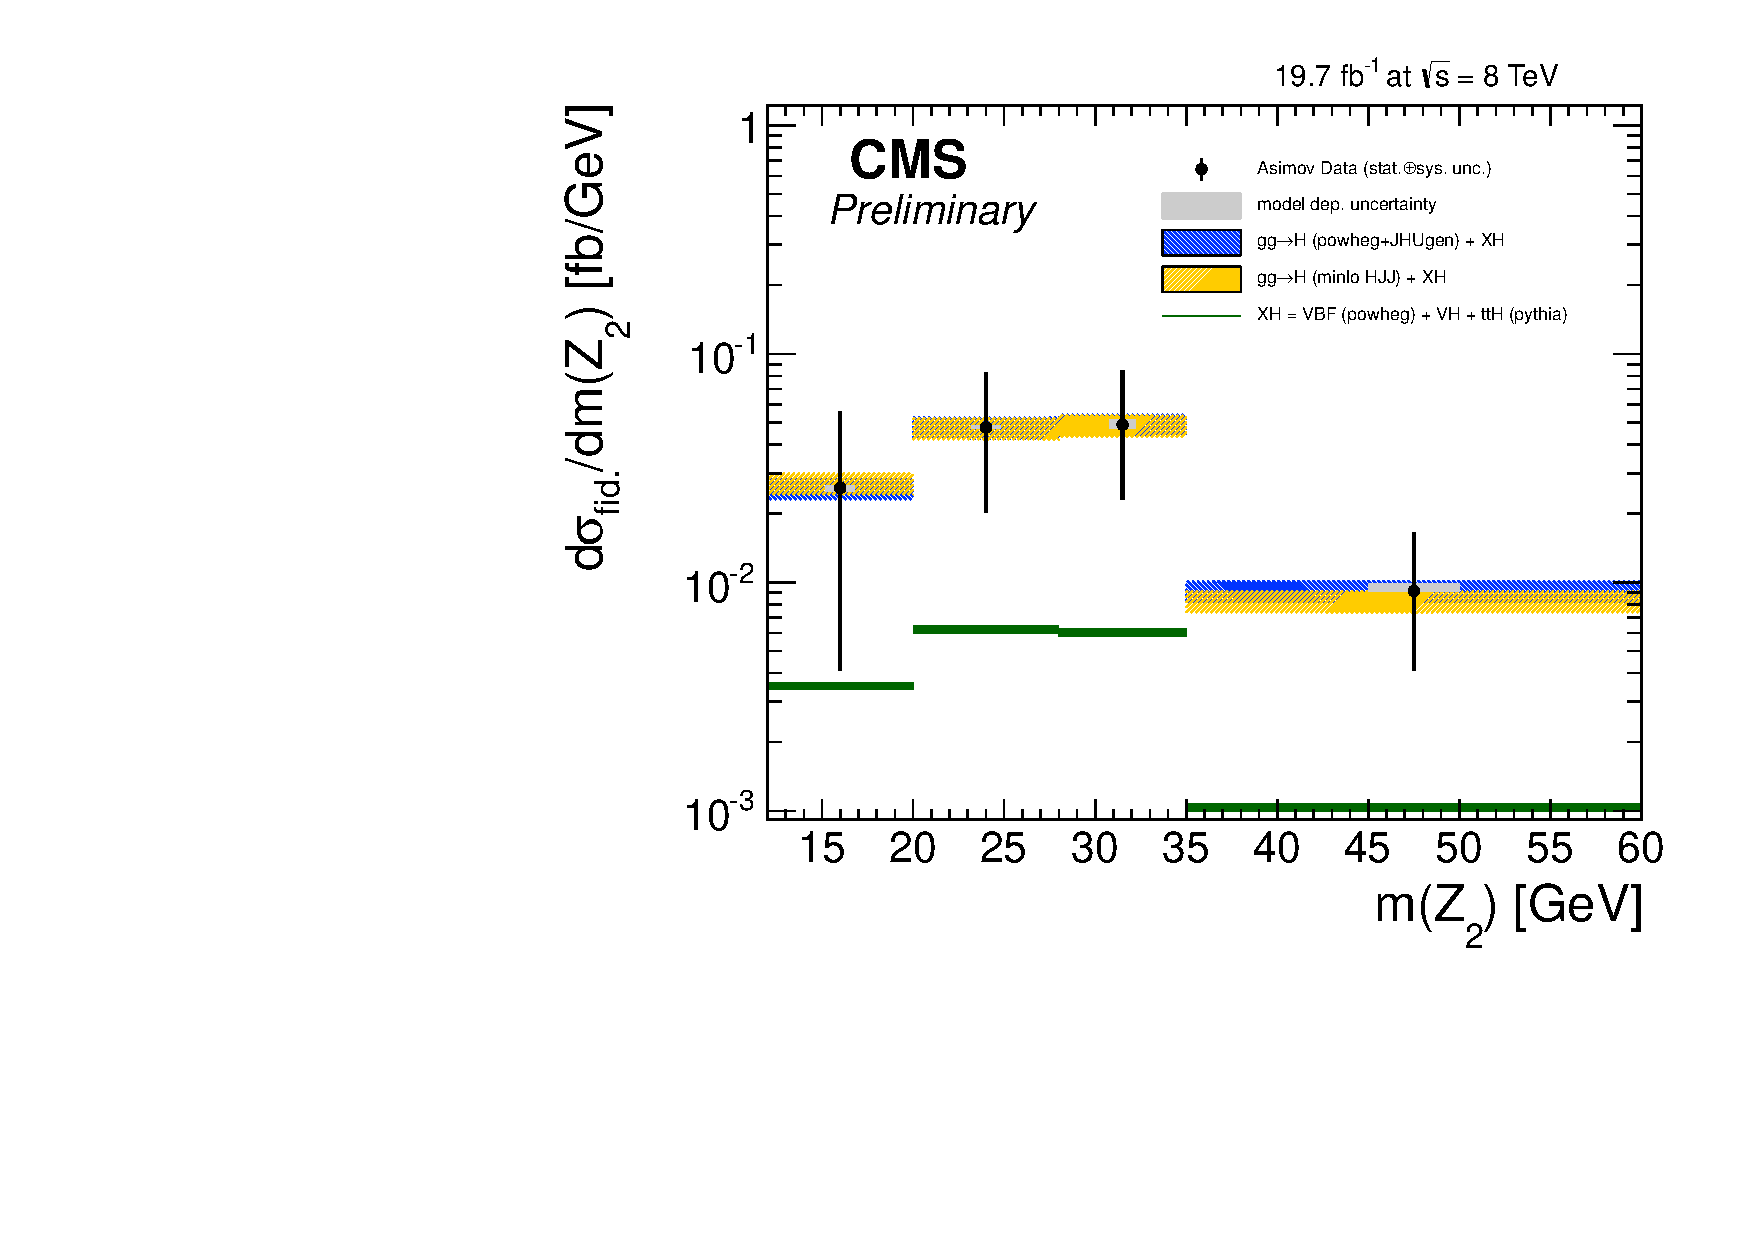
\includegraphics[width=0.42\textwidth,angle=0]{Appendix/Plots/massZ2_unfoldwith_SM_125_logscale.pdf}
      \label{fig:differential-results-asimov:d}
    } \\
    \subfigure[N(jets), $|\eta|<4.7$]{
      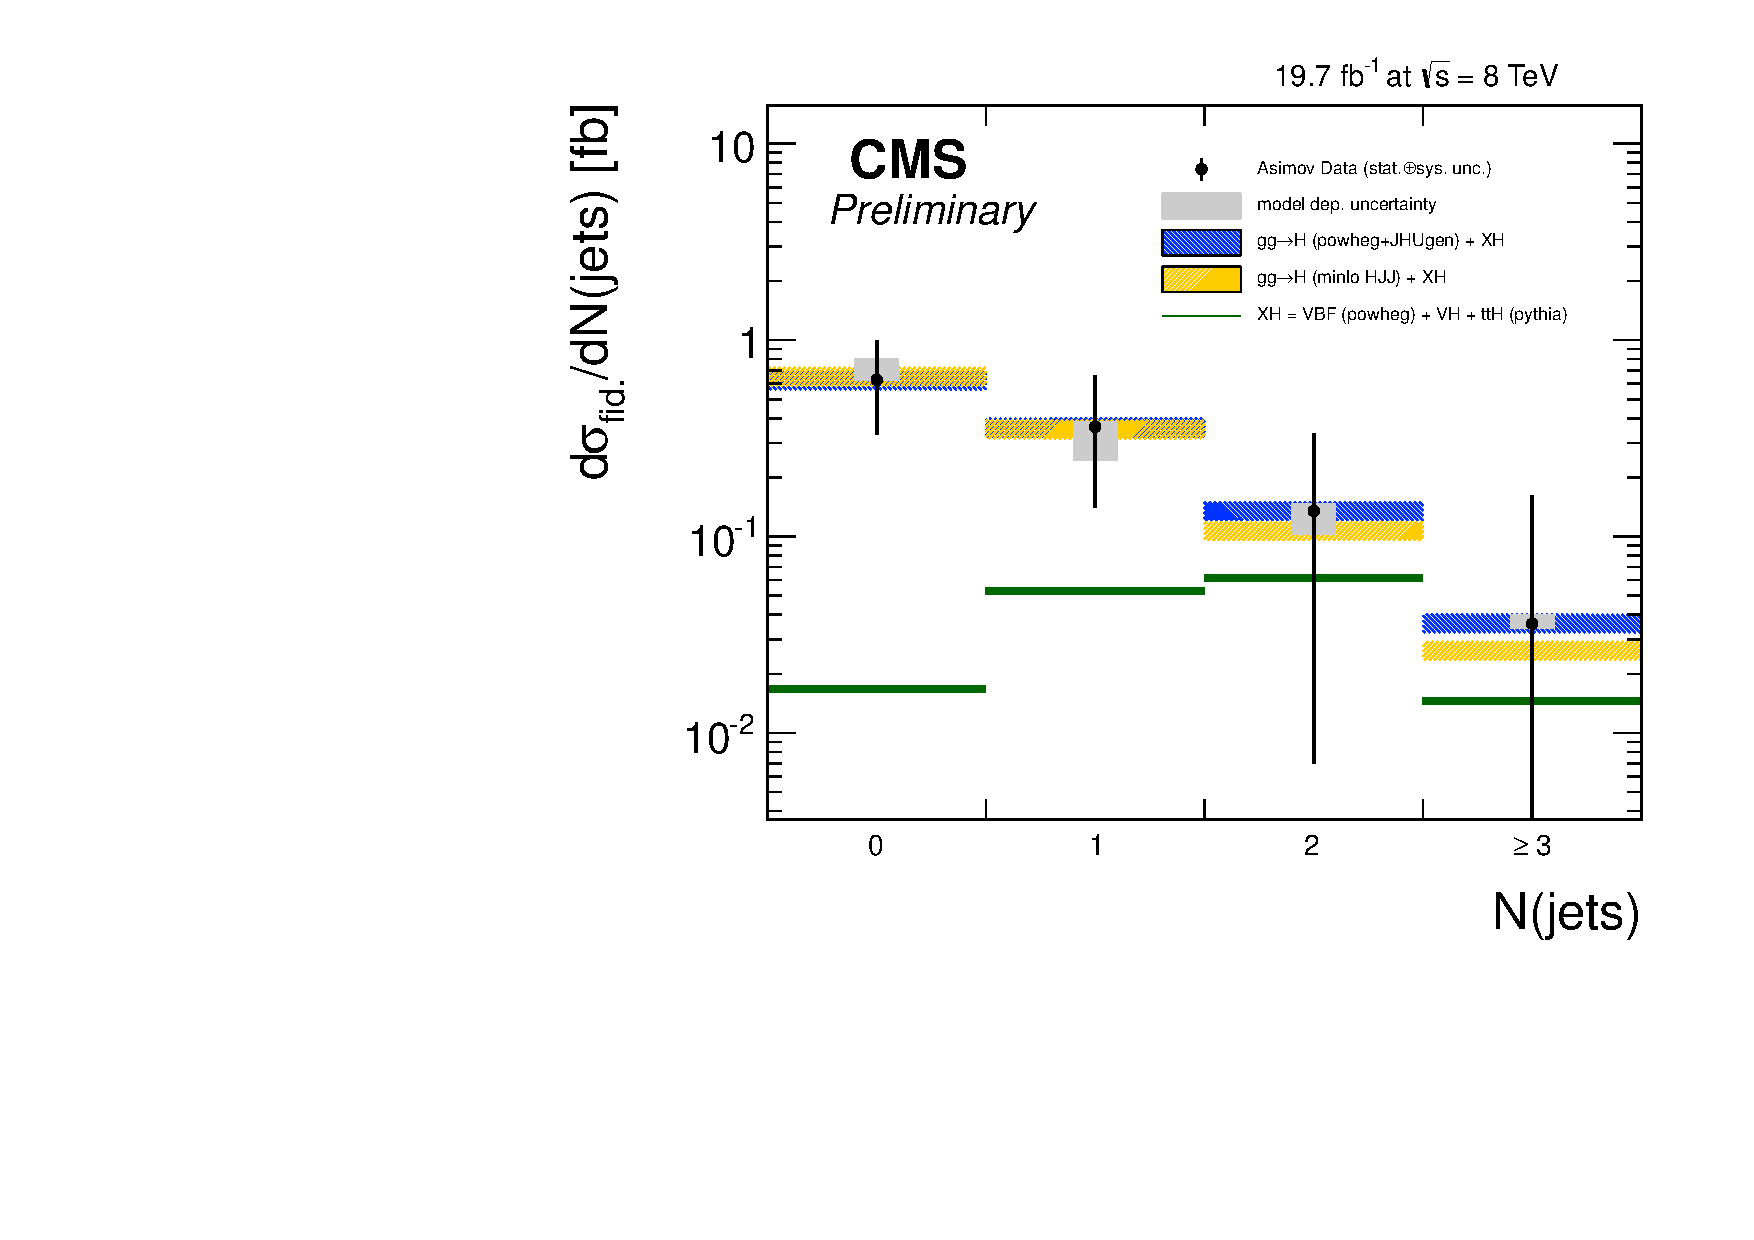
\includegraphics[width=0.42\textwidth,angle=0]{Appendix/Plots/njets_reco_pt30_eta4p7_unfoldwith_SM_125_logscale.pdf}
      \label{fig:differential-results-asimov:e}
    } 
    \subfigure[N(jets), $|\eta|<2.5$]{
      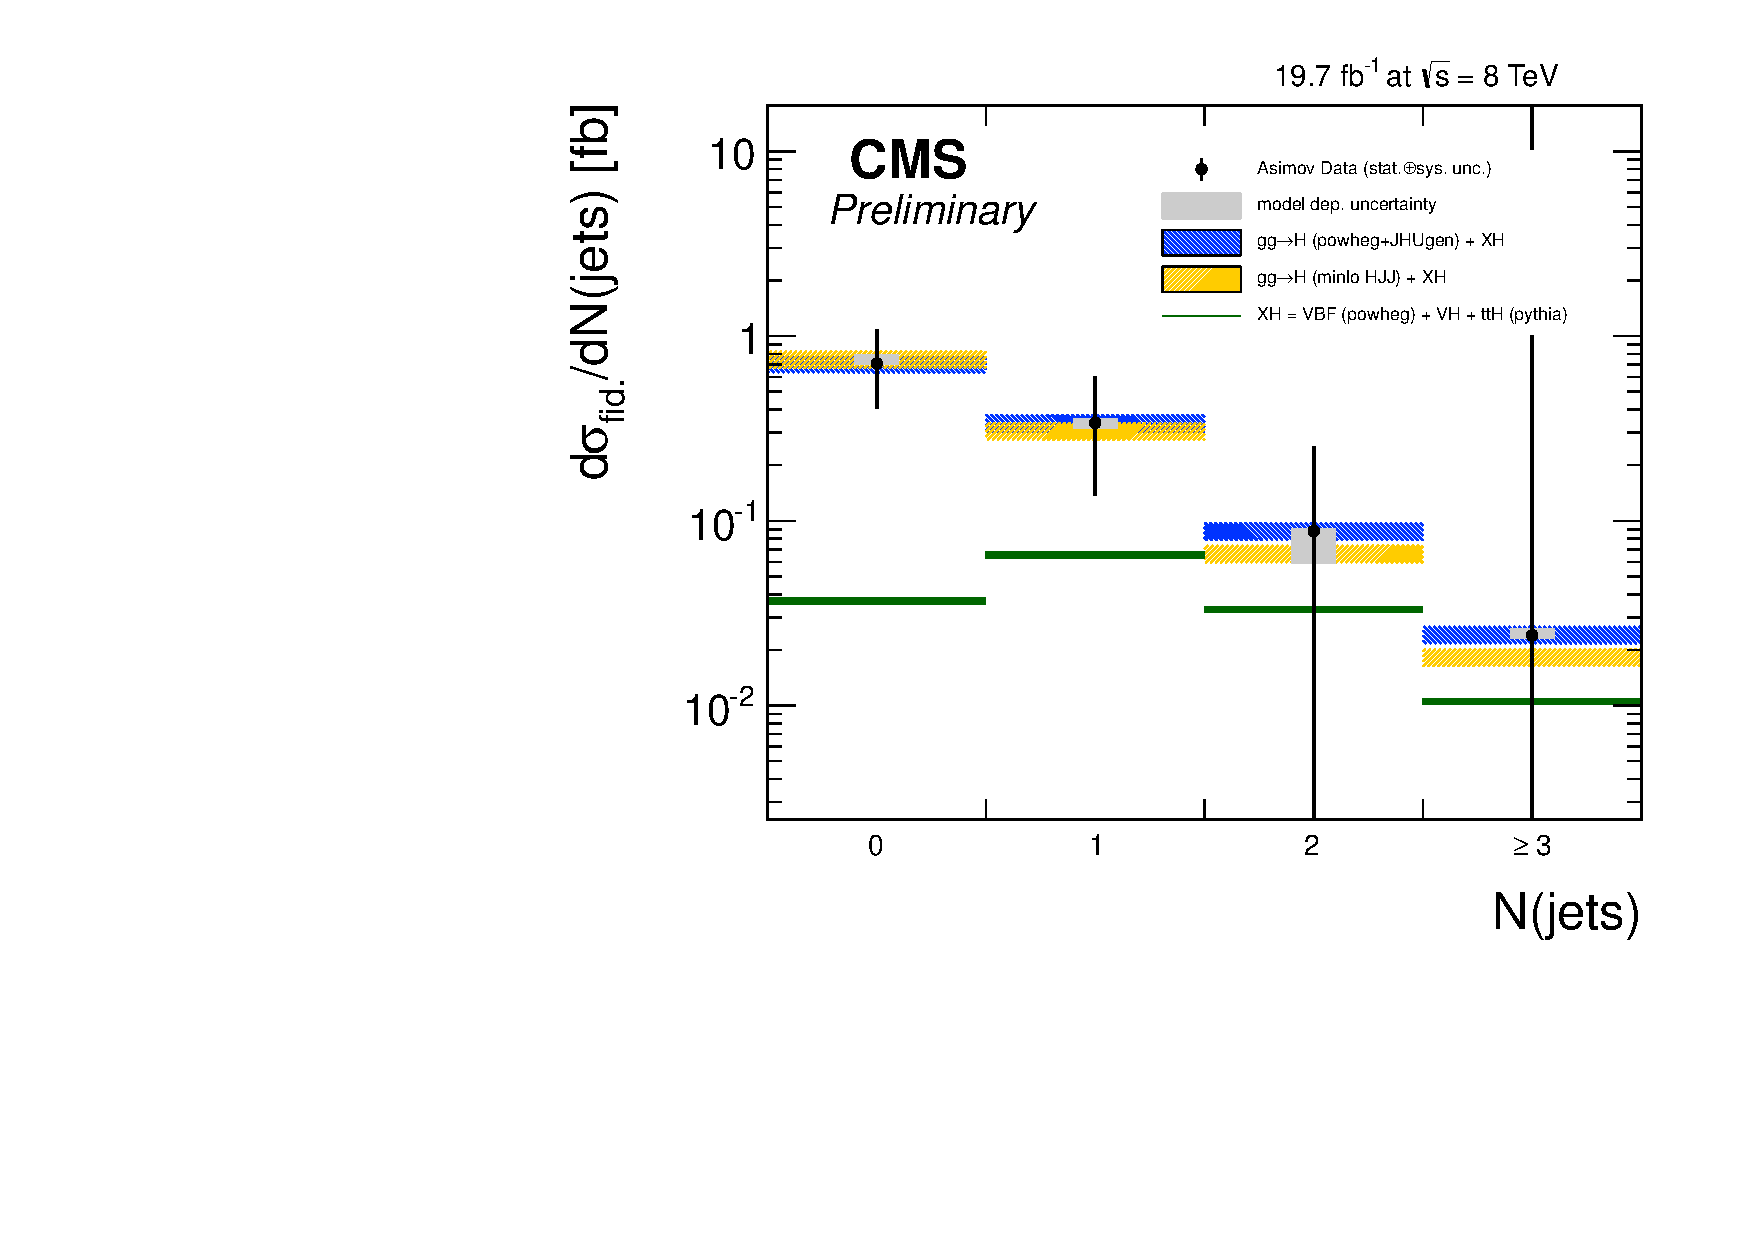
\includegraphics[width=0.42\textwidth,angle=0]{Appendix/Plots/njets_reco_pt30_eta2p5_unfoldwith_SM_125_logscale.pdf}
      \label{fig:differential-results-asimov:f}
    } 
    \caption{Results of the differential cross section measurement for different observables. The predictions where the gg$\rightarrow$H contribution is computed using {\sc powheg+JHUgen} and {\sc minloHJJ} are shown in blue and yellow, respectively. The central value of the measurement is obtained using the efficiencies from the SM where the gg$\rightarrow$H predicition is from {\sc powheg+JHUgen} gg$\rightarrow$H model with m(H)= 125 $\GeV$, and the error bar represents the combined statistical and systematic uncertainty. The grey box represents the additional uncertainty incurred when using different models to unfold the observed data distribution back to particle level. The fraction of $4e,4\mu$ and $2e2\mu$ in each bin is allowed to float in the fit.
    COMMENT: Results shown with Asimov dataset.
    }
  \label{fig:differential-results-asimov}
 \end{center}
\end{figure} 

\begin{figure}[!h!t]
  \begin{center}

    \subfigure[$|\cos \theta_{1}|$]{
      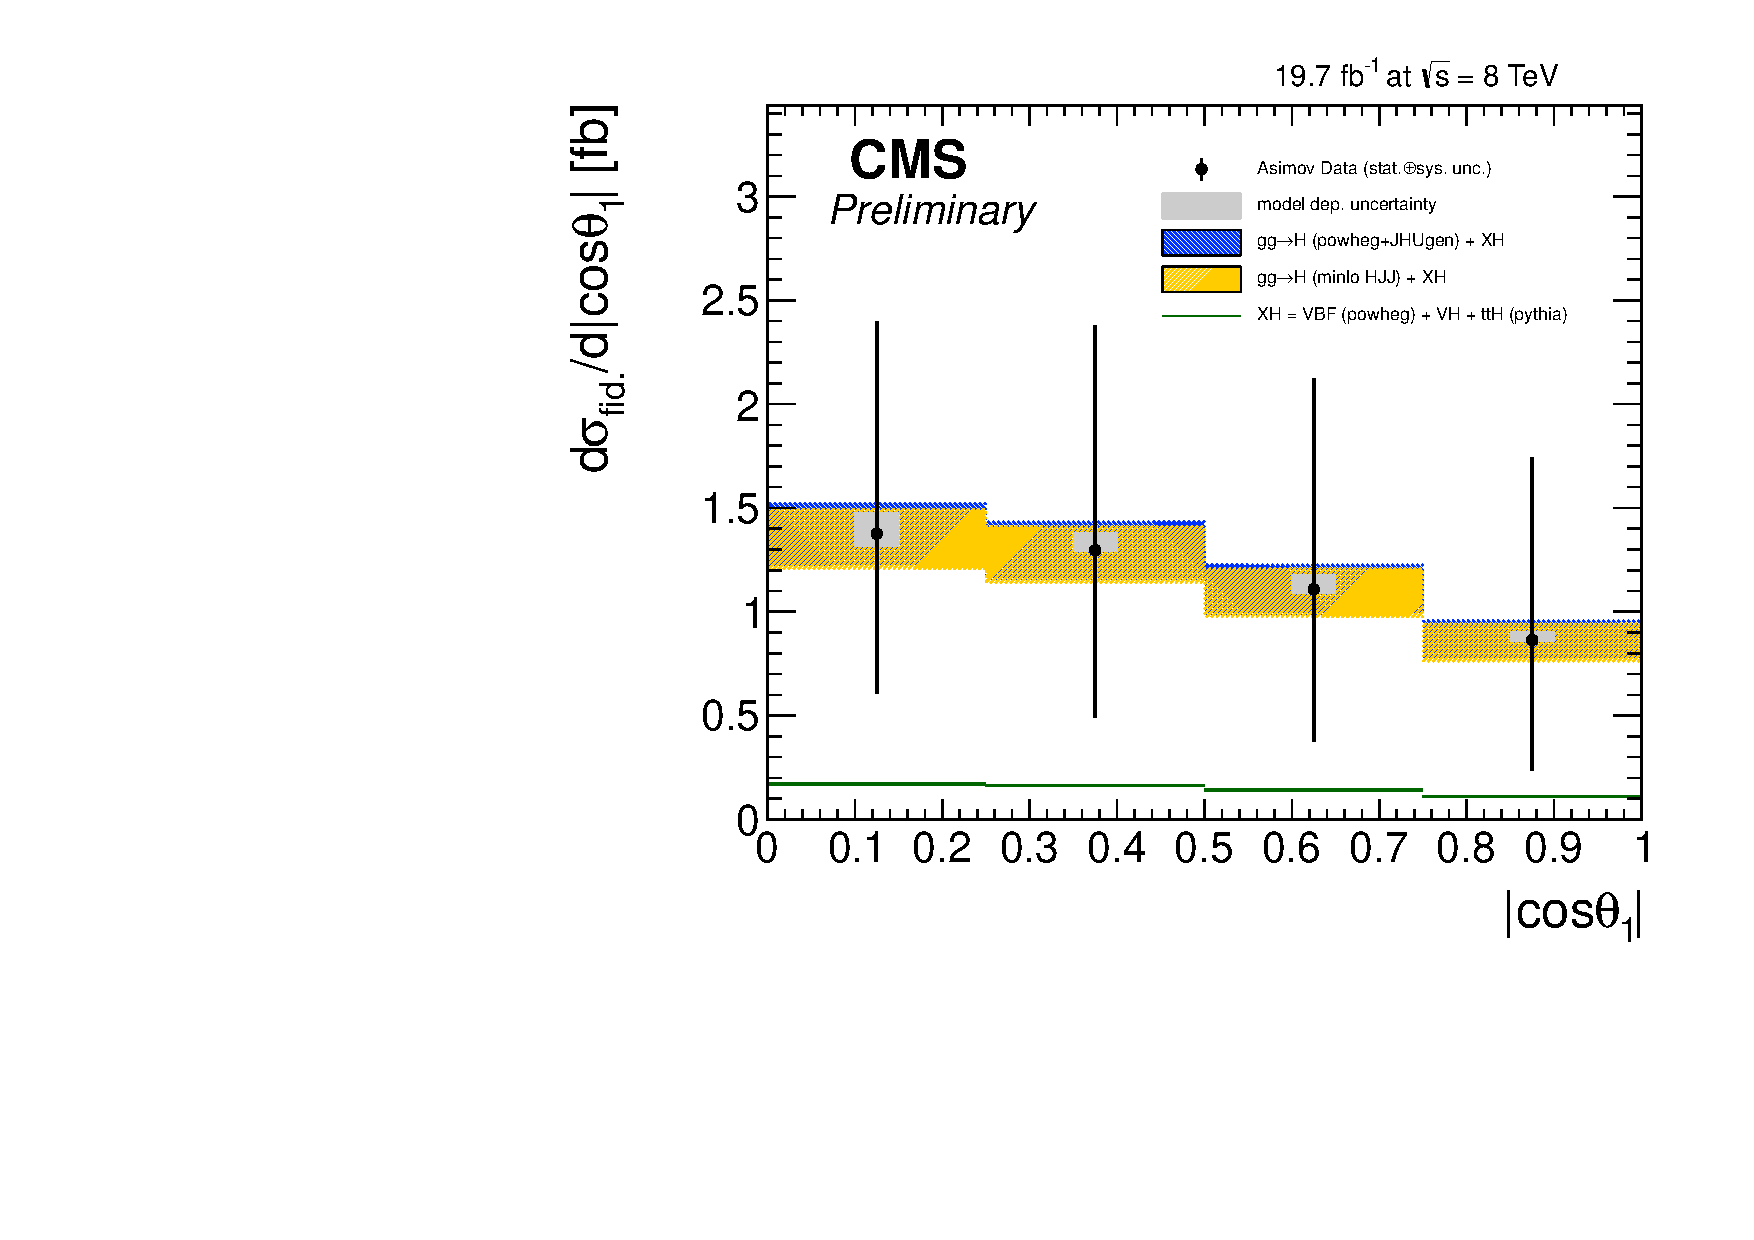
\includegraphics[width=0.42\textwidth,angle=0]{Appendix/Plots/cosTheta1_unfoldwith_SM_125.pdf}
      \label{fig:differential-results-asimov-2:a}
    }
    \subfigure[$|\cos \theta_{2}|$]{
      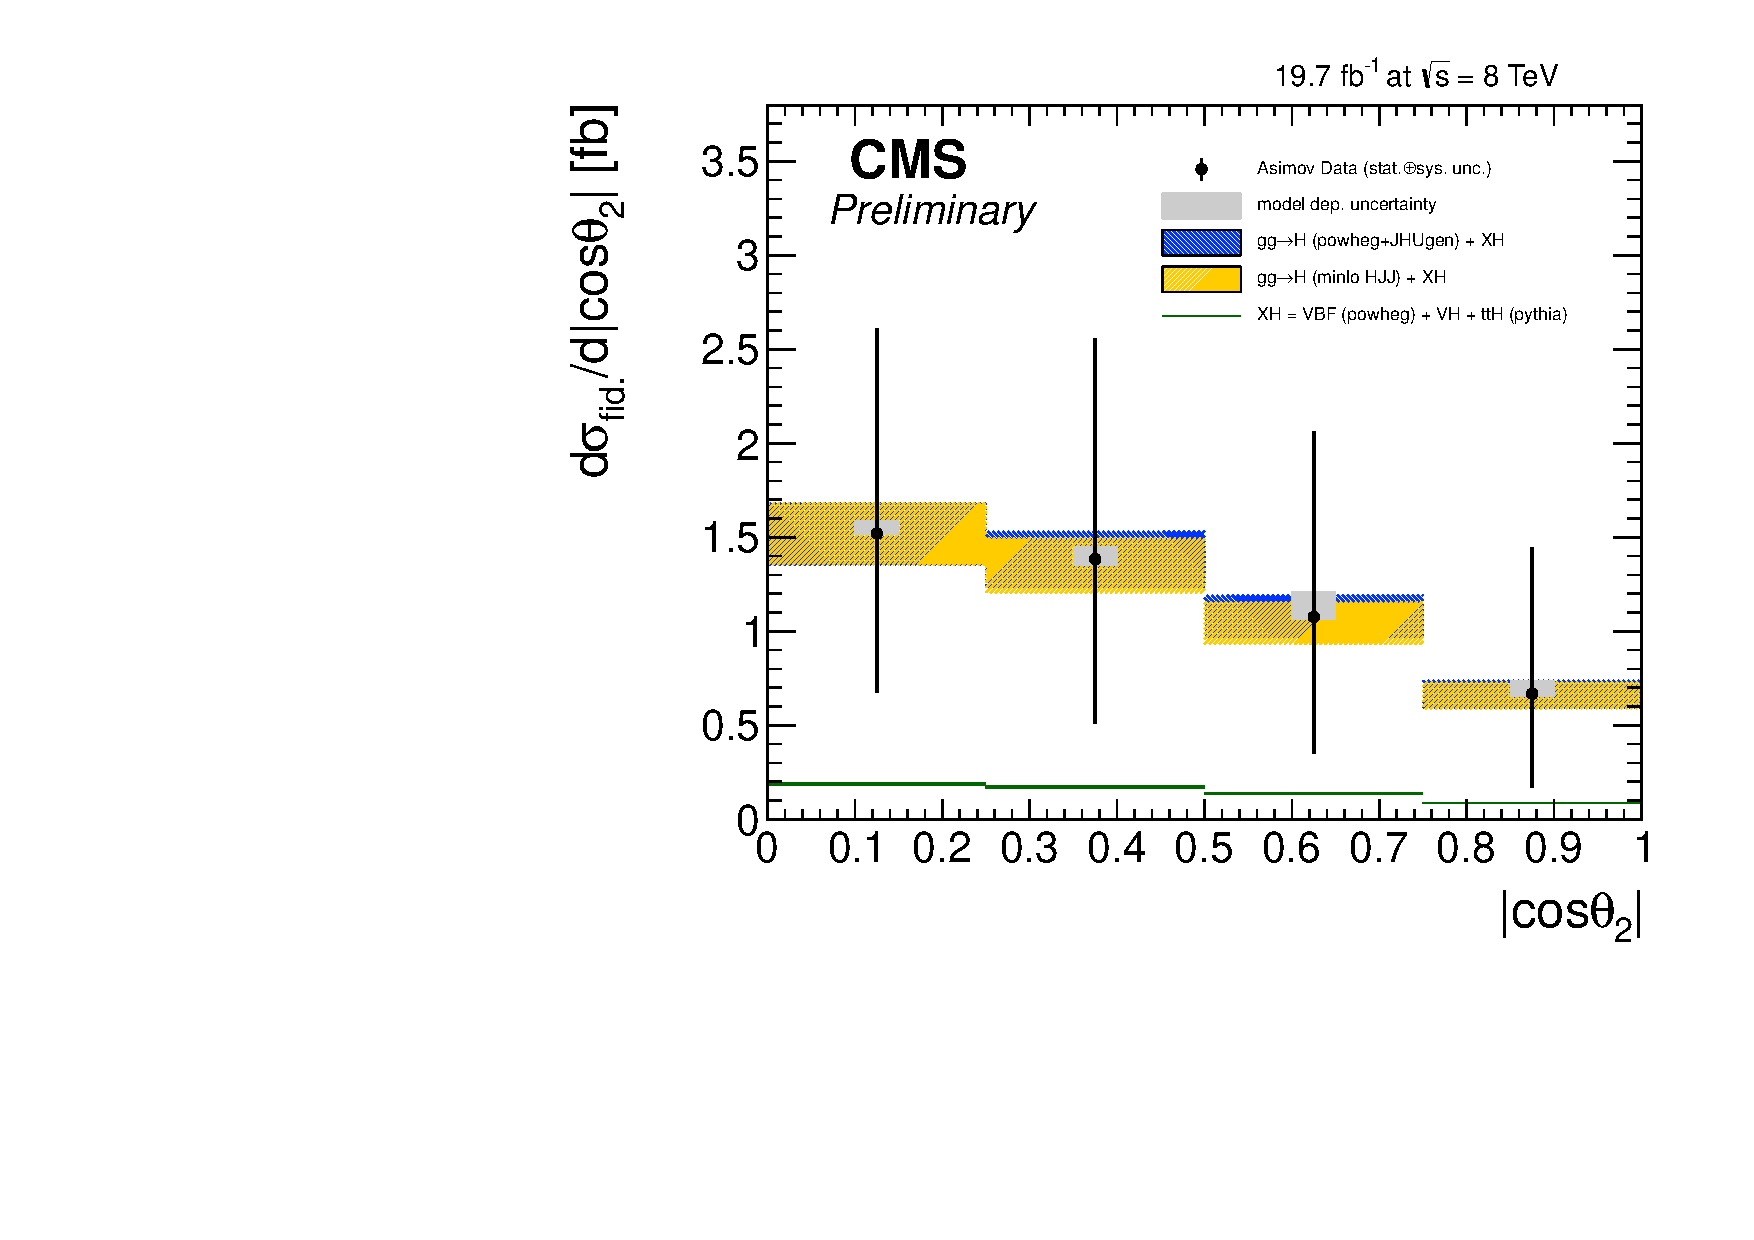
\includegraphics[width=0.42\textwidth,angle=0]{Appendix/Plots/cosTheta2_unfoldwith_SM_125.pdf}
      \label{fig:differential-results-asimov-2:b}
    } \\
    \subfigure[$|\Phi|$]{
      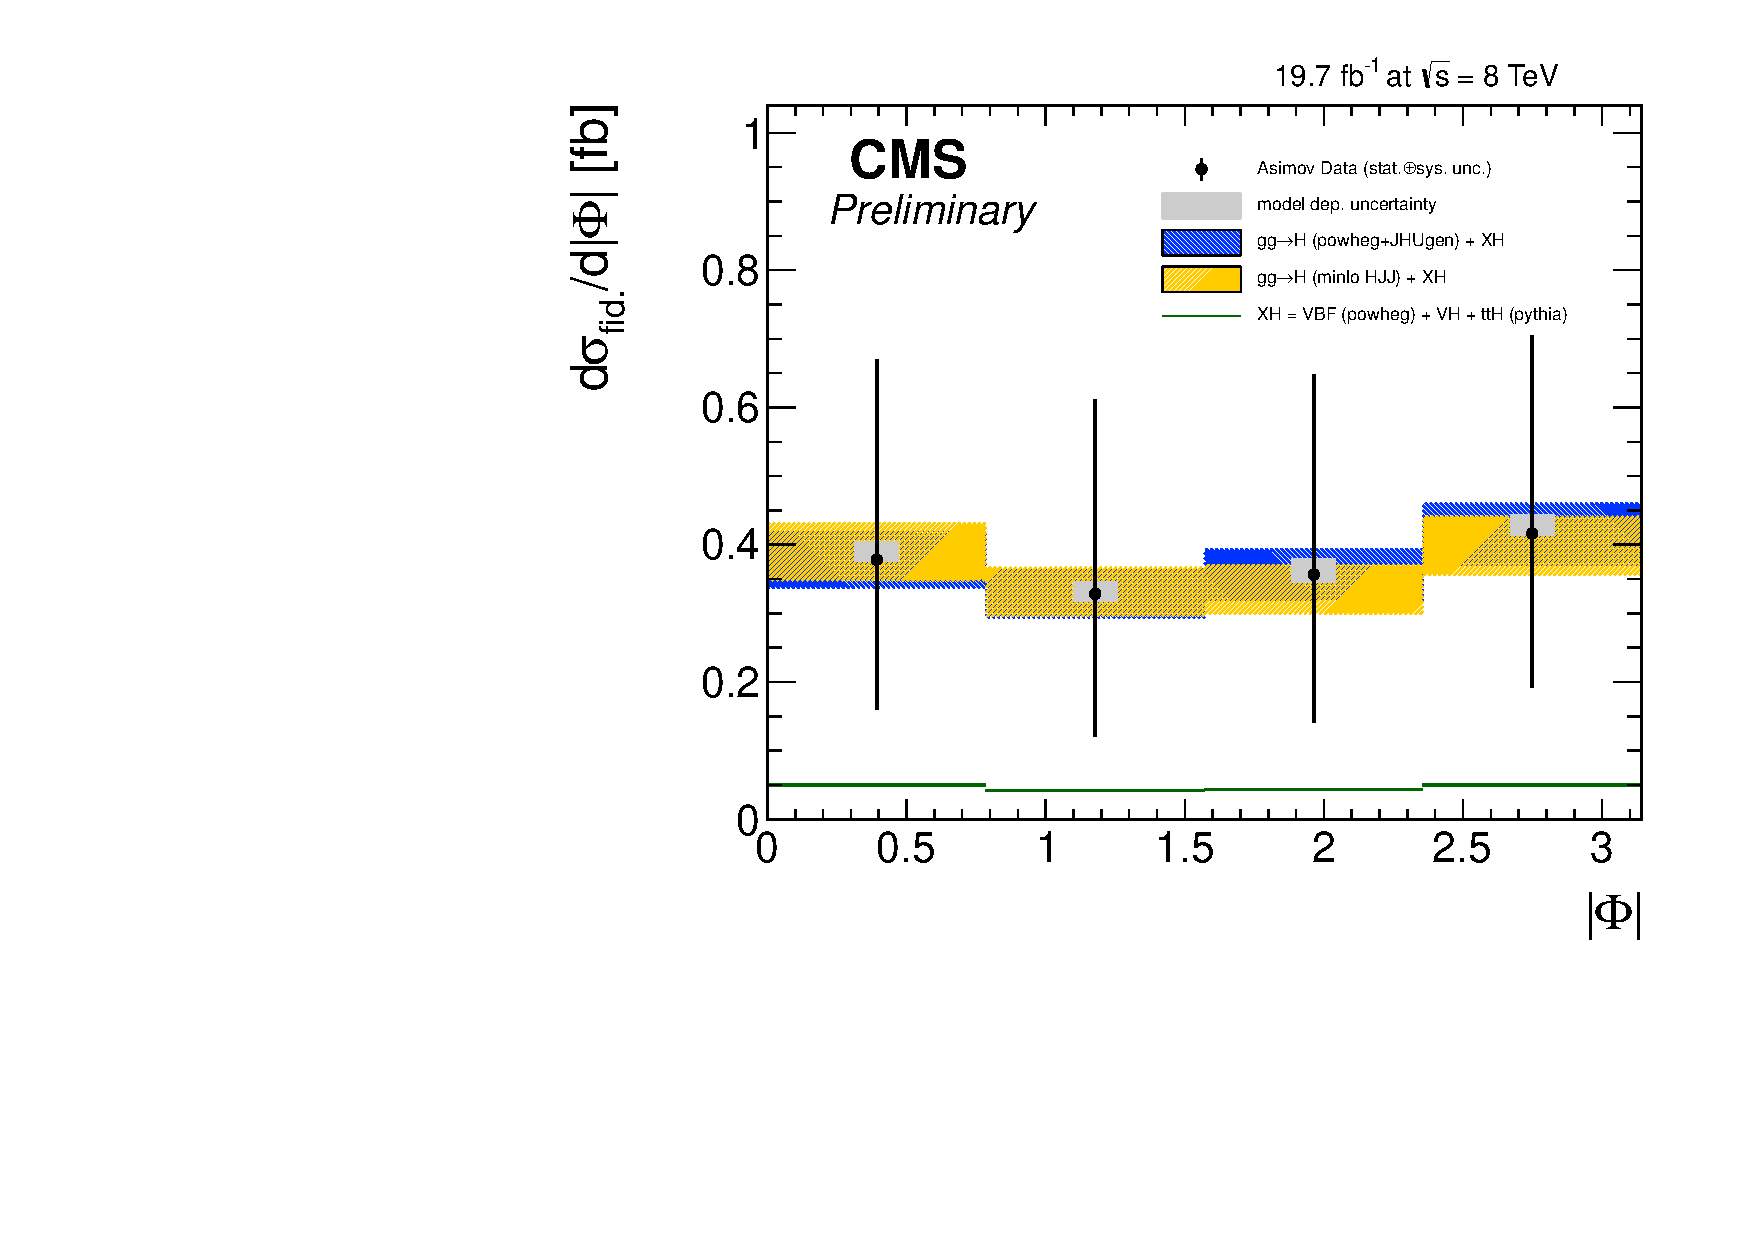
\includegraphics[width=0.42\textwidth,angle=0]{Appendix/Plots/Phi_unfoldwith_SM_125.pdf}
      \label{fig:differential-results-asimov-2:c}
    } 
    \subfigure[$|\Phi_{1}|$]{
      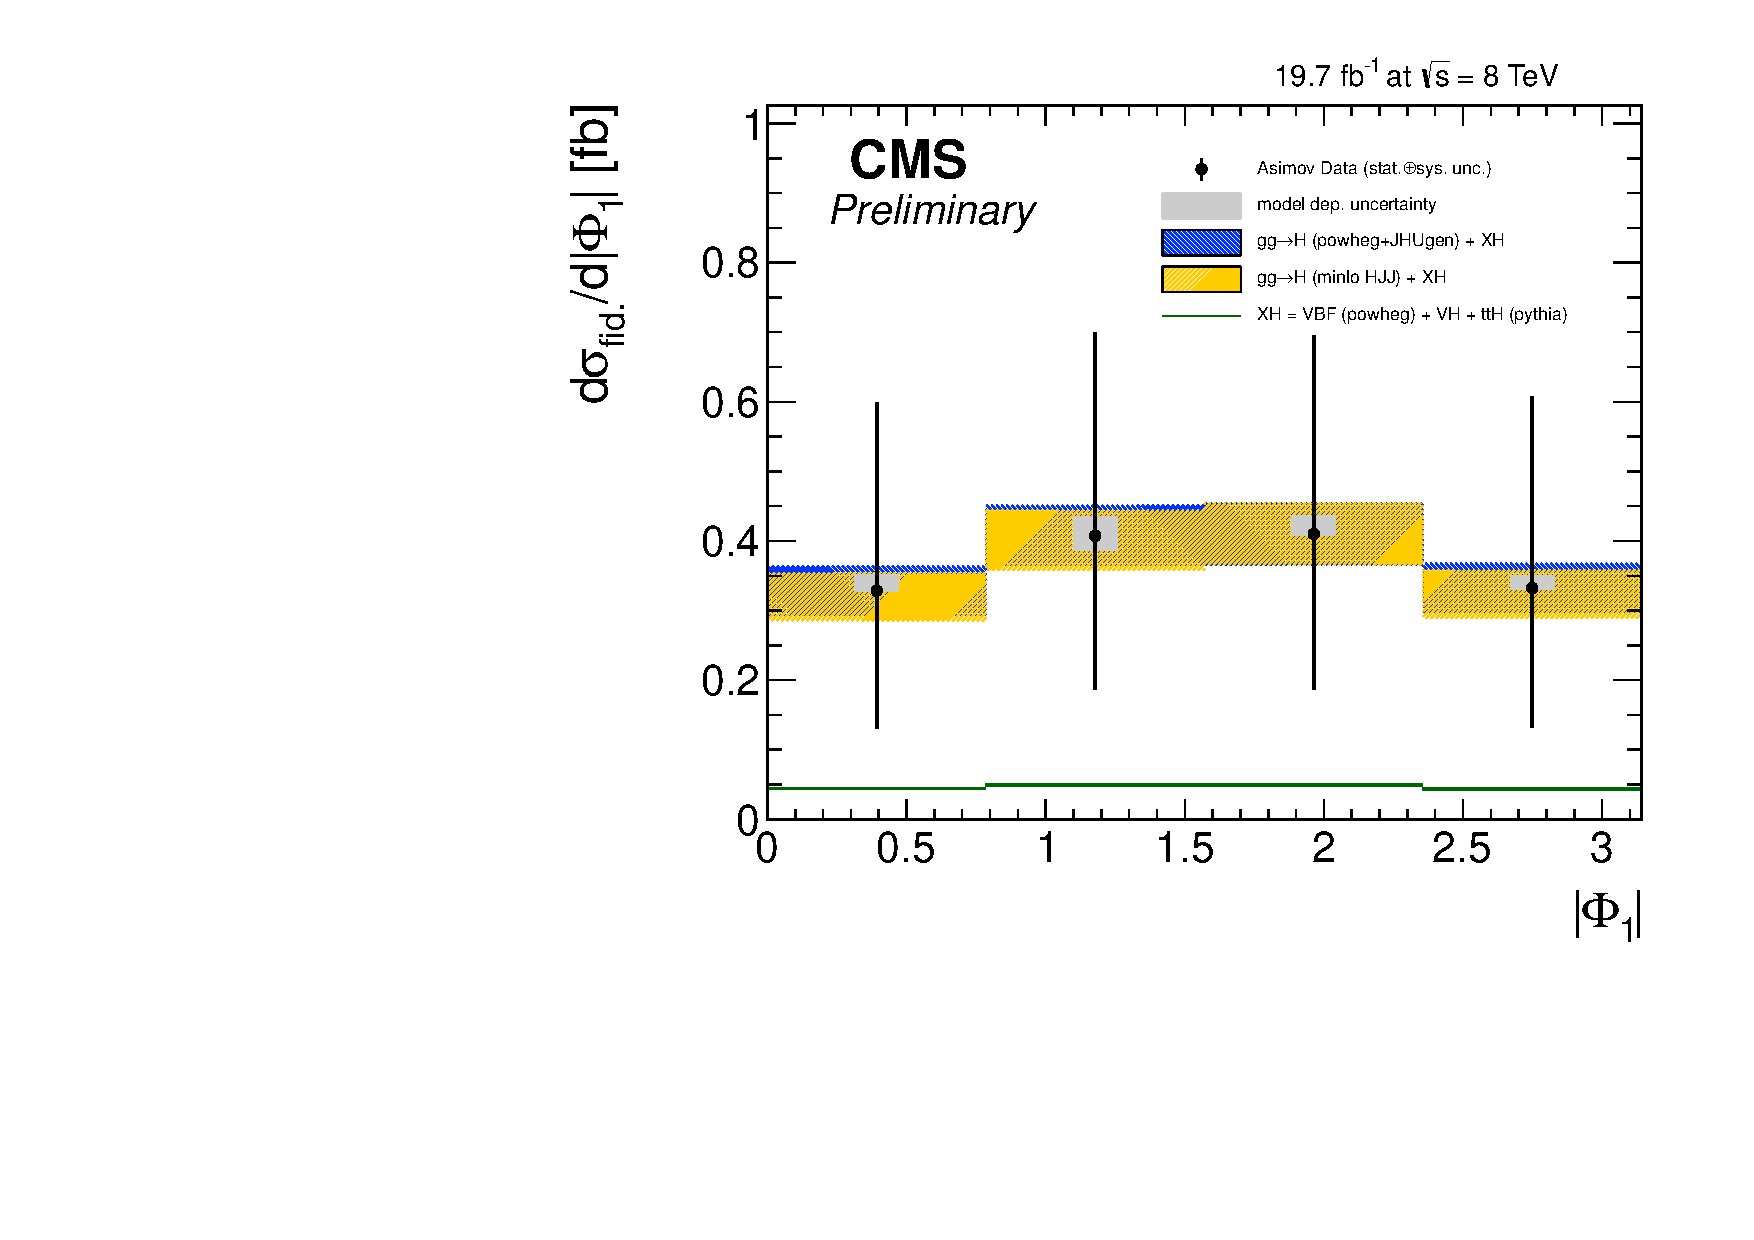
\includegraphics[width=0.42\textwidth,angle=0]{Appendix/Plots/Phi1_unfoldwith_SM_125.pdf}
      \label{fig:differential-results-asimov-2:d}
    } \\
    \subfigure[$|\cos \theta^{*}|$]{
      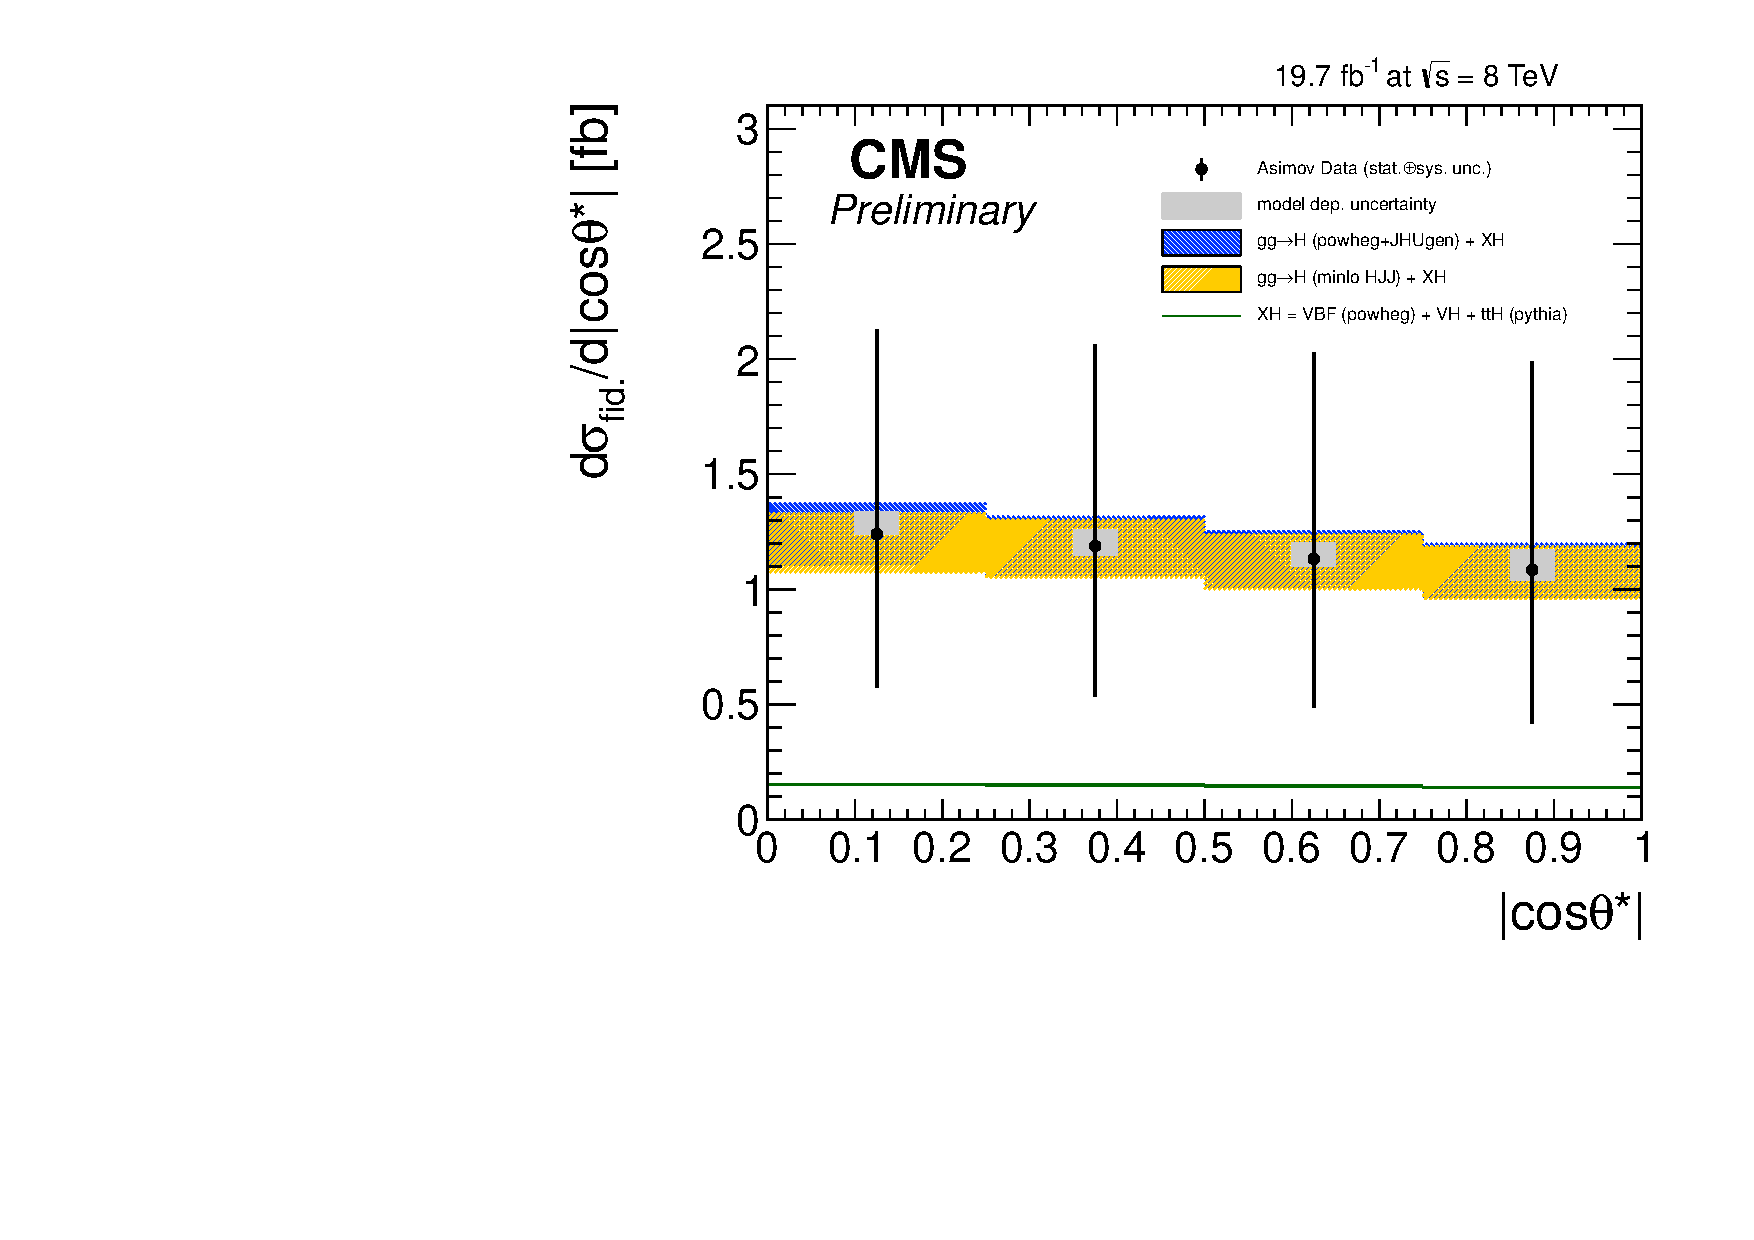
\includegraphics[width=0.42\textwidth,angle=0]{Appendix/Plots/cosThetaStar_unfoldwith_SM_125.pdf}
      \label{fig:differential-results-asimov-2:e}
    }
    \caption{Results of the differential cross section measurement for different observables. The predictions where the gg$\rightarrow$H contribution is computed using {\sc powheg+JHUgen} and {\sc minloHJJ} are shown in blue and yellow, respectively. The central value of the measurement is obtained using the efficiencies from the SM where the gg$\rightarrow$H predicition is from {\sc powheg+JHUgen} gg$\rightarrow$H model with m(H)= 125 $\GeV$, and the error bar represents the combined statistical and systematic uncertainty. The grey box represents the additional uncertainty incurred when using different models to unfold the observed data distribution back to particle level. The fraction of $4e,4\mu$ and $2e2\mu$ in each bin is allowed to float in the fit.
    COMMENT: Results shown with Asimov dataset.
    }
  \label{fig:differential-results-asimov-2}
 \end{center}
\end{figure}

\begin{figure}[!h!tb]
  \begin{center}

    \subfigure[$\pt(\mathrm{Z})$]{
      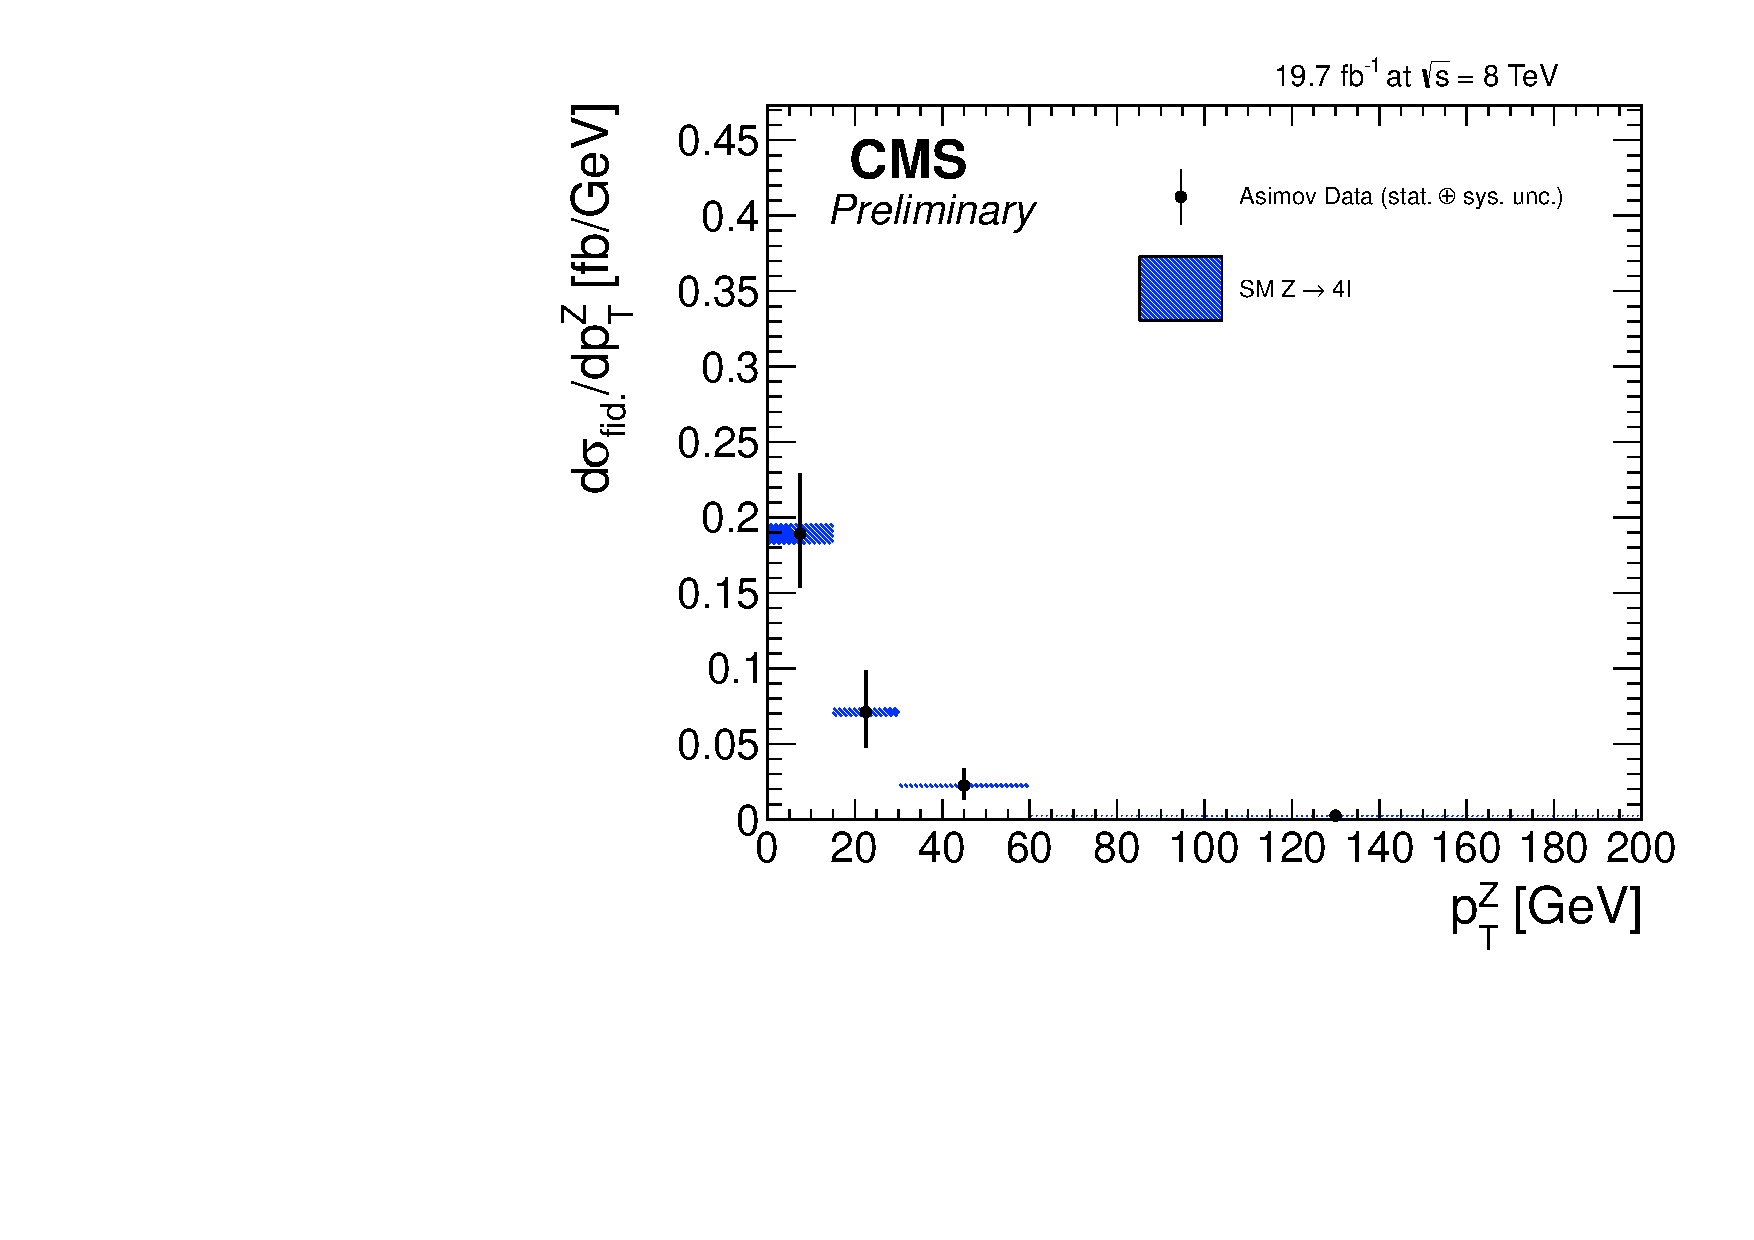
\includegraphics[width=0.42\textwidth,angle=0]{Appendix/Plots/pT4l_Asimov_unfoldwith_SMZ4l.pdf}
      \label{fig:differential-results-asimov-Z4l:a}
    }
    \subfigure[$|y(\mathrm{Z})|$]{
      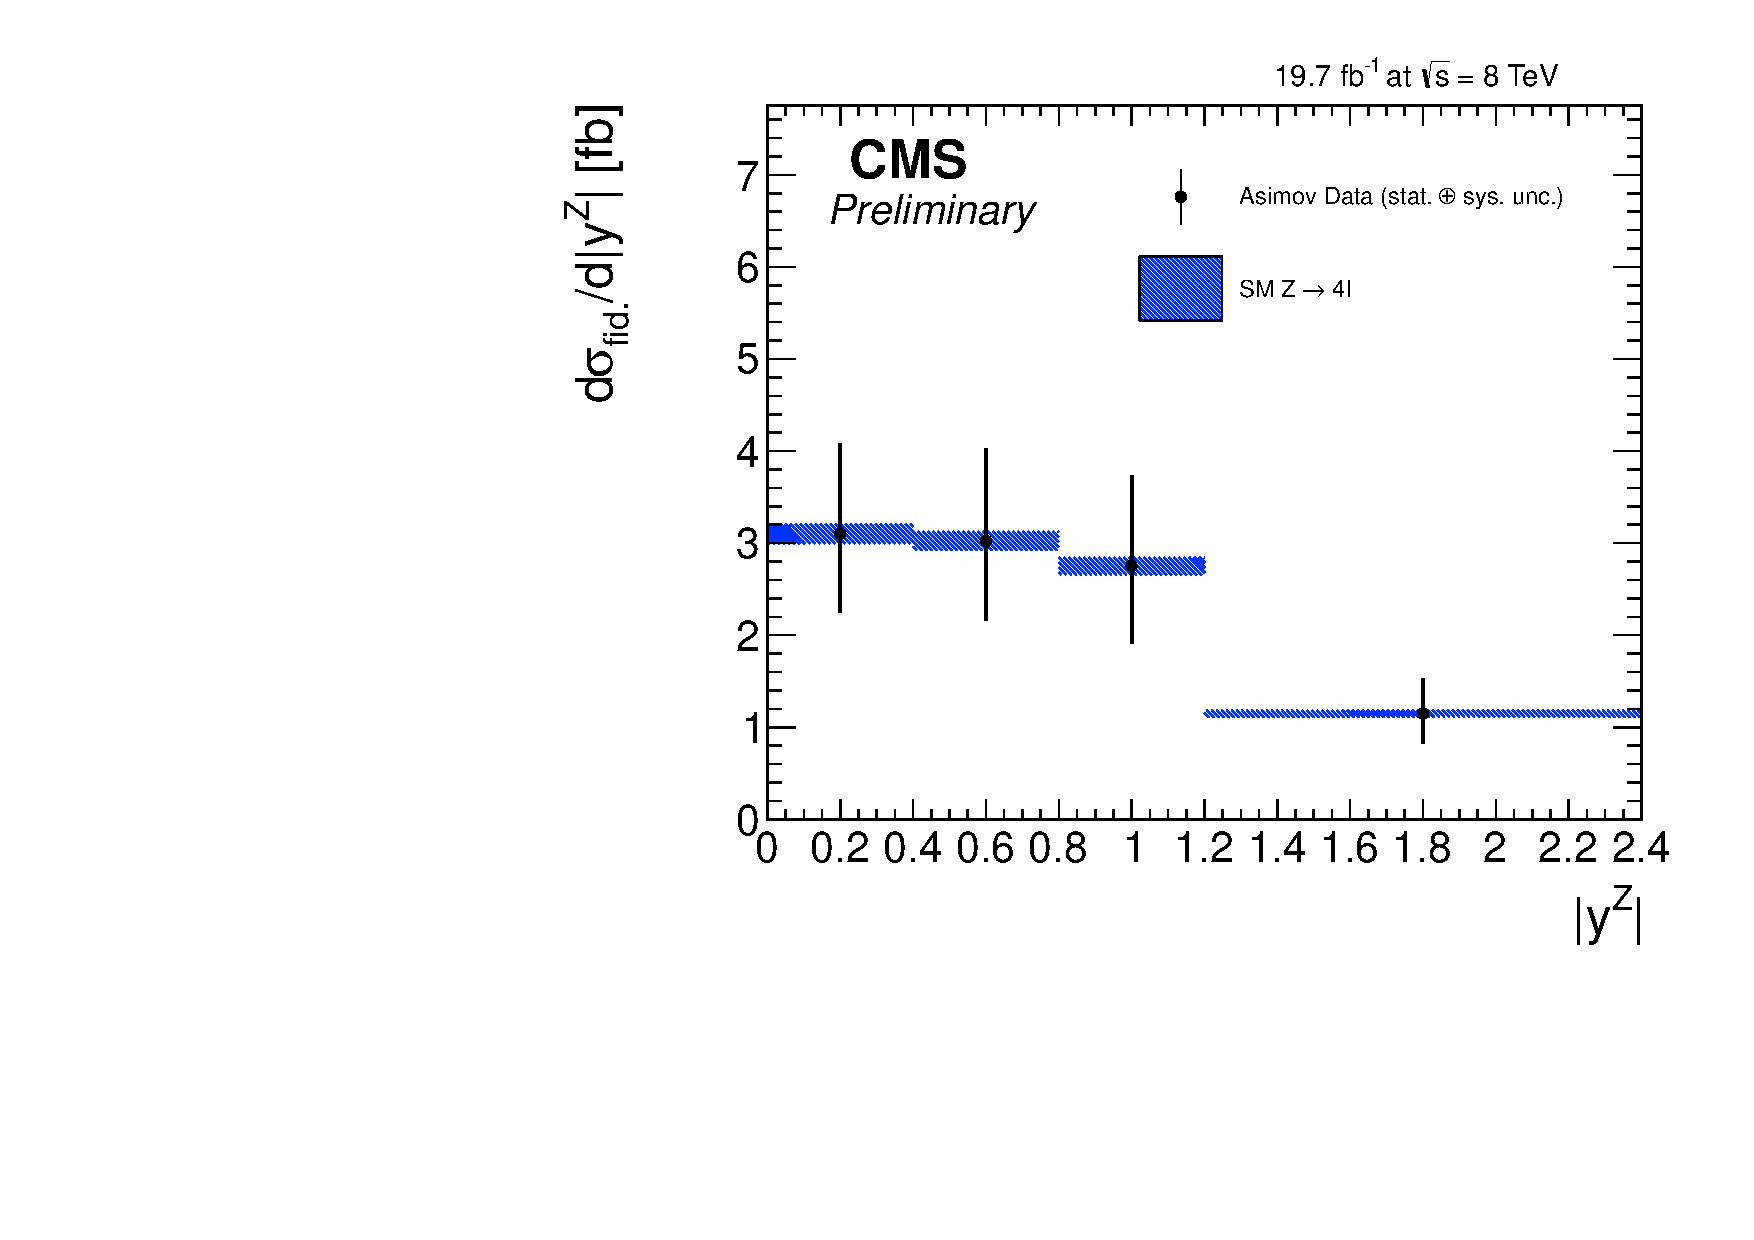
\includegraphics[width=0.42\textwidth,angle=0]{Appendix/Plots/rapidity4l_Asimov_unfoldwith_SMZ4l.pdf}
      \label{fig:differential-results-asimov-Z4l:c}
    } \\
    \subfigure[N(jets)]{
      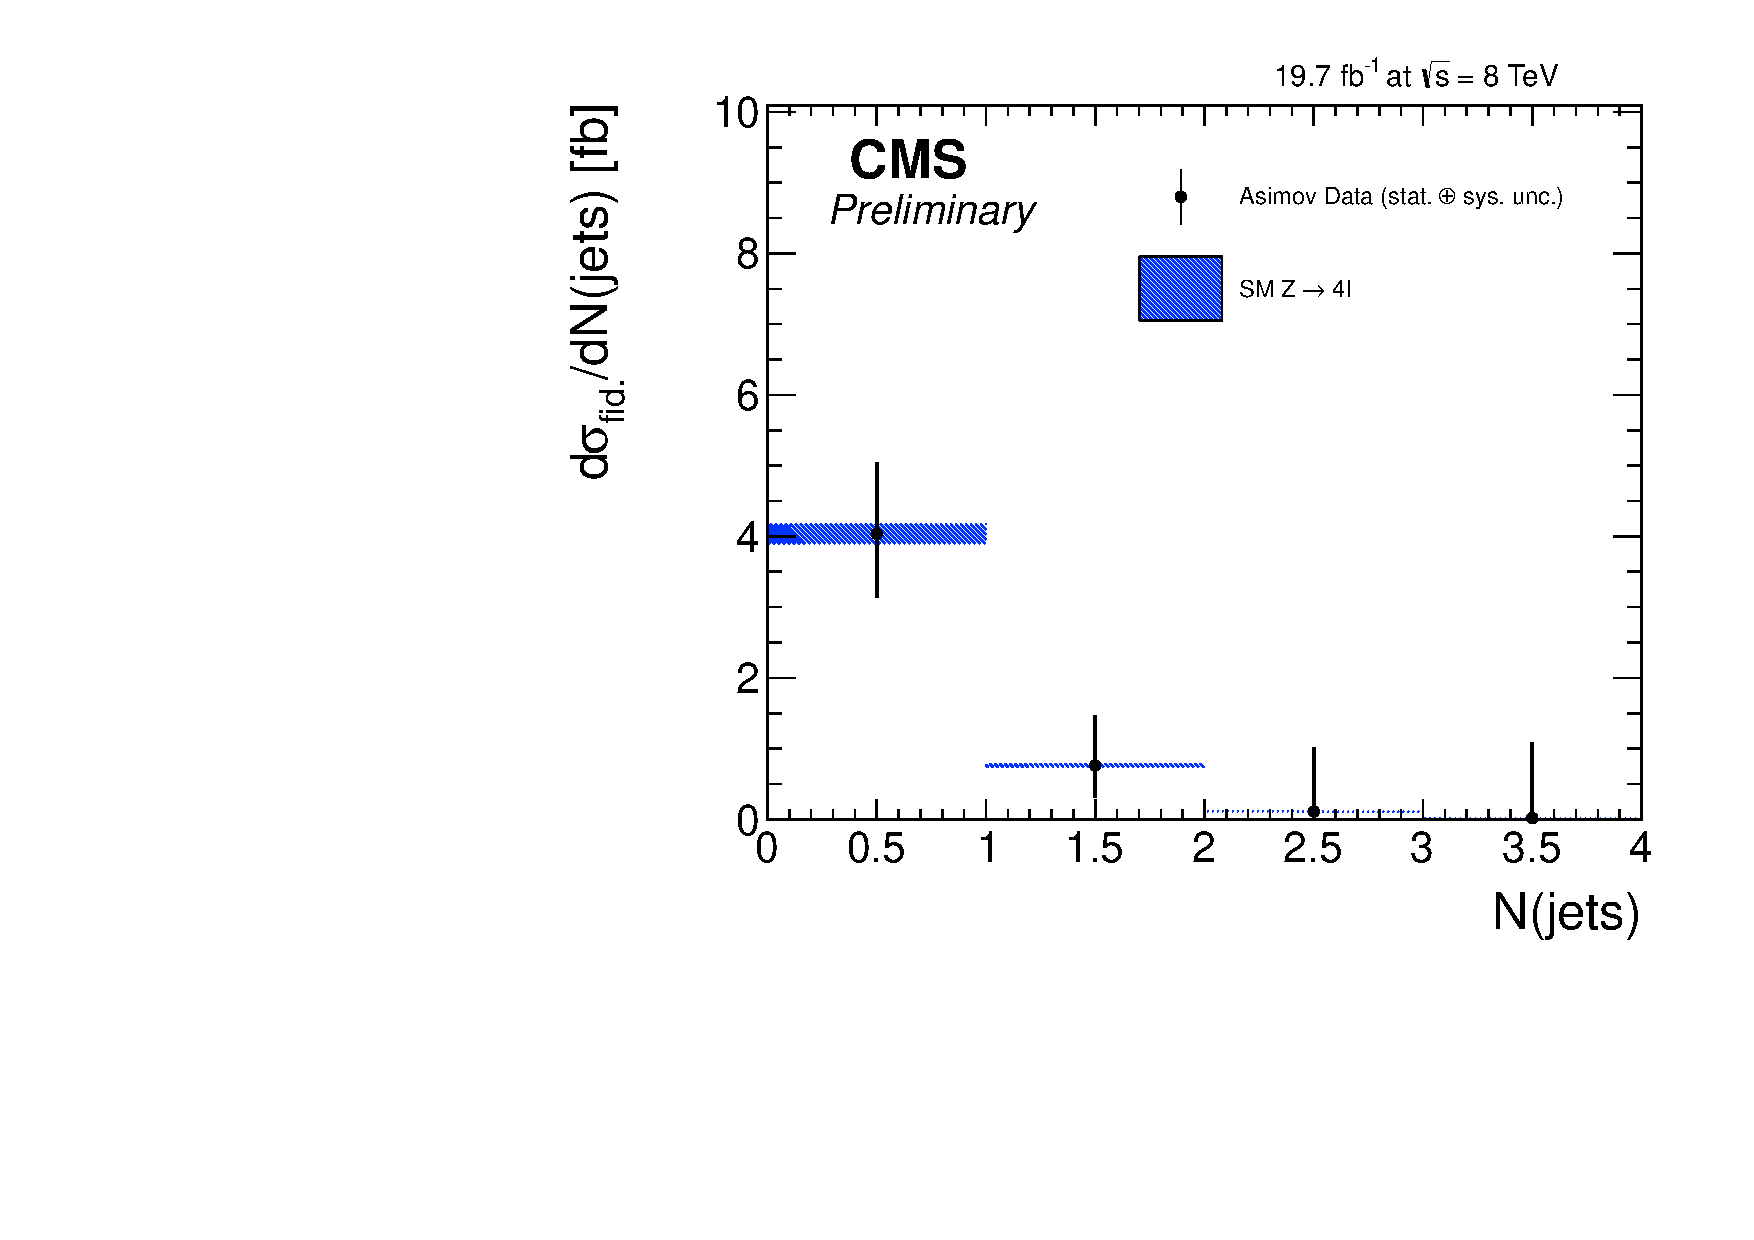
\includegraphics[width=0.42\textwidth,angle=0]{Appendix/Plots/njets_reco_pt30_eta4p7_Asimov_unfoldwith_SMZ4l.pdf}
      \label{fig:differential-results-asimov-Z4l:e}
    }
    \subfigure[$\mathrm{m}(\mathrm{Z}_{2})$]{
      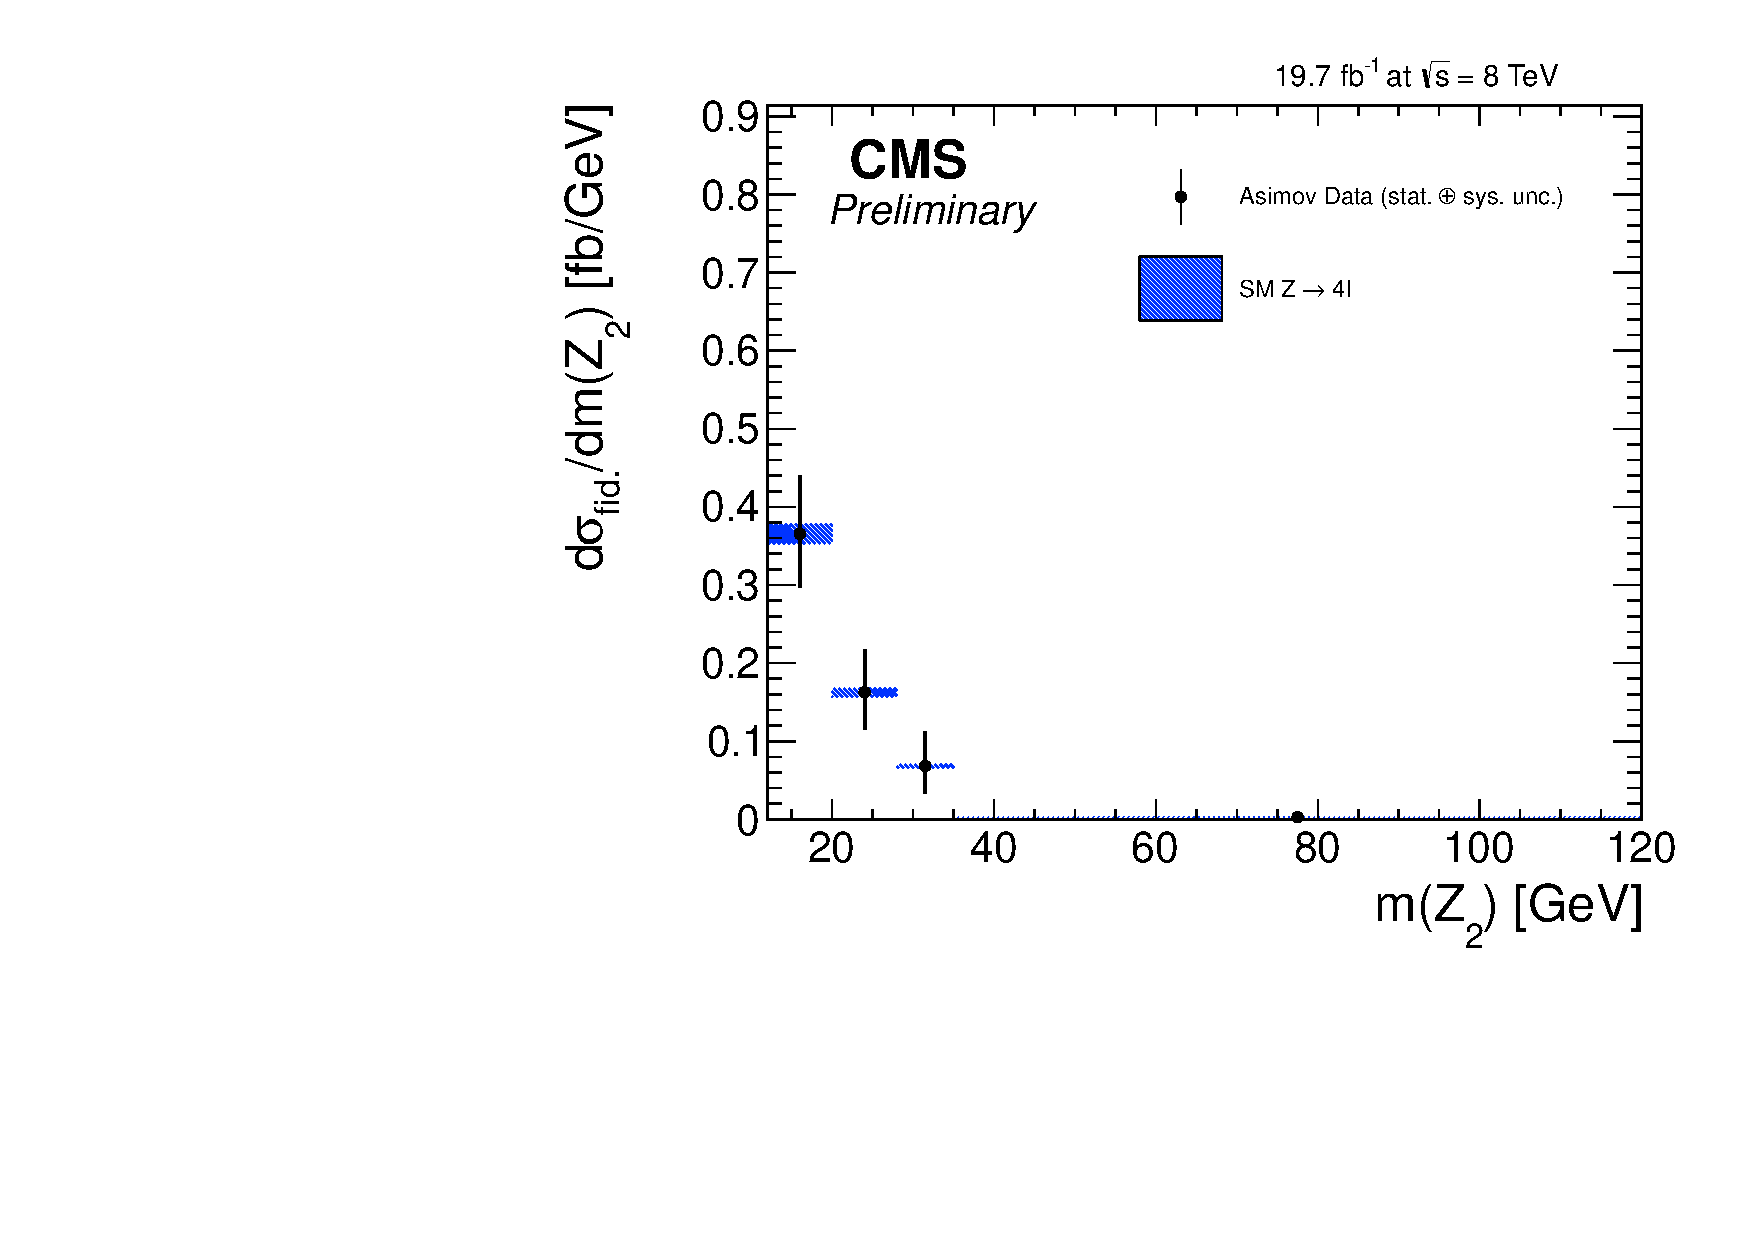
\includegraphics[width=0.42\textwidth,angle=0]{Appendix/Plots/massZ2_Asimov_unfoldwith_SMZ4l.pdf}
      \label{fig:differential-results-asimov-Z4l:b}
    } \\
    \subfigure[$|\cos \theta^{*}|$]{
      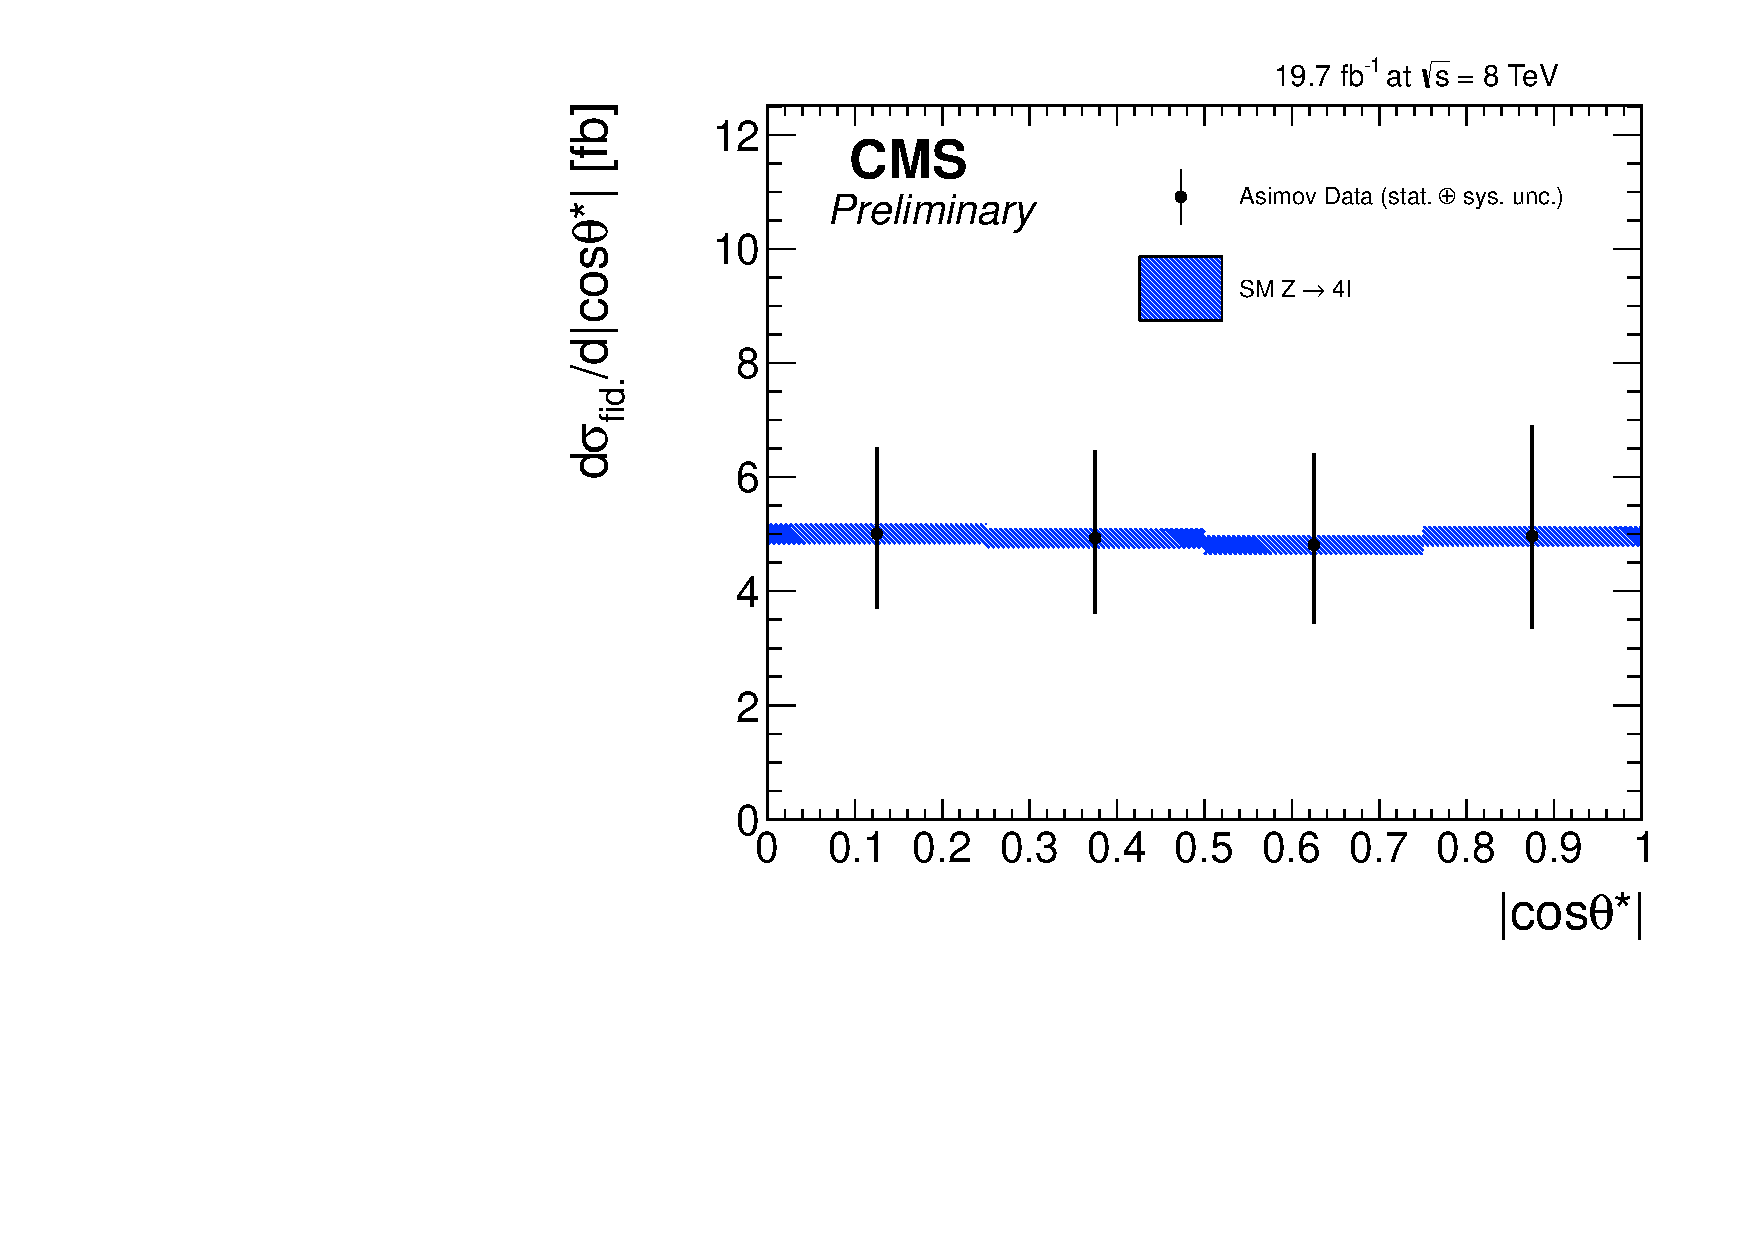
\includegraphics[width=0.42\textwidth,angle=0]{Appendix/Plots/cosThetaStar_Asimov_unfoldwith_SMZ4l.pdf}
      \label{fig:differential-results-asimov-Z4l:d}
    }
    \caption{Results of the Z$\rightarrow 4 \ell$ differential cross section measurement for different observables. The predictions from {\sc powheg} are shown in blue. The error bar represents the combined statistical and systematic uncertainty. The fraction of $4e,4\mu$ and $2e2\mu$ in each bin is allowed to float in the fit.
    COMMENT: Results shown with Asimov dataset.
    }
  \label{fig:differential-results-asimov-Z4l}
 \end{center}
\end{figure}

